\documentclass{main}
 

\usepackage{graphicx}      % include this line if your document contains figures
\usepackage{natbib}        % required for bibliography
\usepackage{enumerate}
\usepackage[utf8]{inputenc}
\usepackage{graphicx}
\usepackage{float}
\usepackage[centerlast,small,sc]{caption} 
\setlength{\captionmargin}{30pt}
\usepackage[brazilian]{babel}
\usepackage[none]{hyphenat} 
\usepackage{subcaption} 
\usepackage{capt-of}
\usepackage{kpfonts} 
\usepackage{stackengine}
\usepackage{calc}
\newlength\shlength
\newcommand\xshlongvec[2][0]{\setlength\shlength{#1pt}%
  \stackengine{-5.6pt}{$#2$}{\smash{$\kern\shlength%
    \stackengine{7.55pt}{$\mathchar"017E$}%
      {\rule{\widthof{$#2$}}{.57pt}\kern.4pt}{O}{r}{F}{F}{L}\kern-\shlength$}}%
      {O}{c}{F}{T}{S}}
\sloppy  

\begin{document}

\begin{frontmatter}

\title{Estudo do conceito para metodologia e revestimento robótico
de turbinas \textit{in situ} - EMMA
\thanksref{footnoteinfo}} 

\thanks[footnoteinfo]{This work is supported by ESBR under contract COPPETEC
JIRAU 09/15 6631-0003/2015 (ANEEL R\&D program).}

\author[1]{Renan S. Freitas}
\author[1]{Gabriel Alcantara C. S.}
\author[1]{Eduardo Elael M. S.}
\author[1]{Estevão Fróes}
\author[1]{Ramon R. Costa}
\author[2]{Sylvain Joyeux}
\author[2]{Patrick M. Paranhos}

  \address[1]{Departamento de Engenharia Elétrica, COPPE UFRJ, Rio de Janeiro,
  Brasil} 
  % TODO Renan: Verificar departamento do patrick e sylvain
  \address[2]{Centro de Inovação em Robótica (CIR), Rio de Janeiro, Brasil}
  
\begin{abstract}                % Abstract of not more than 250 words.
%TODO Renan: Resumo
\end{abstract} 
 
\begin{keyword}
%TODO Renan: Keywords
\end{keyword}

\end{frontmatter}

%\section{Introdução}
%TODO Renan: Introdução
Hydropower is the most mature, reliable and cost-effective
renewable power generation technology available \citep{brown}, accouting 16
percent of global electricity generation. The global hydropower use and
capacity will increase about 3.1\% each year for the next 25 years \citep{wi}.
The total investment for large-scale hydropower projects
typically range from USD 1000/kW to around USD 3500/kW and, once commissioned,
the annual operation and maintenance costs of hydropower plants are often
quoted as 4\% of the investment per kW per year \citep{ecofys}. 

In the specific case of Brazil, the third biggest hydroelectric potential of
the world, hydropower represents 84\% of its electric power total production.
Brazil is the second biggest country of installed hydropower capacity, 84 GW,
and in the Amazon basin, in Madeira river, this number will be increased next
years by the construction of Santo Antonio (3150 MW) and Jirau (3300 MW) power
plants. The dependance on this renewable power source mobilizes private
initiative investments on research centers and universities, and motivates the
development systems with a high degree of automation based on advanced robotic
systems \citep{aneel}.

A major challenge for hydropower companies is\ldots


 


In this paper, we present the state of the art in\ldots

%a general overview of the
%ROSA robot, and a detailed description of the embedded electronics, power
% supply system and software architecture. The robot is designed to perform monitoring and inspection
%tasks of the stoplogs' stacking and retrieving process in a power
%plant. Carrying different sensors, the robot analyses sensor data \emph{in
%loco} or stores it for a posterior analysis, interprets the results, and
%sends specific data to the operator. The sensors can identify the lifting beam
%actual operation (stack/retrieve), stoplog attachment/detachment, the
%lifting beam inclination, the system depth in water, and a
%profiling sonar for sediments inspection. 

%This text is organized as follows: the state of the art general overview of the
%robot and its main challenges are presented in Section \ref{sec:sota}, detailed
%descriptions of the embedded electronics, the vehicle support system, power
%supply system, and software architecture are taken in
%Sections \ref{sec:electronics_overview}, \ref{sec:powersupply_overview}, and
%\ref{sec:software} respectively.
%In Section \ref{sec:results}, preliminary results are shown, and concluding
%remarks are drawn in Section \ref{sec:conclusions}. 
\section{Descrição do problema}\label{sec::consideracoes}

O fenômeno de cavitação e abrasão em hidroturbinas provoca redução da eficiência
na geração de energia e desgaste superficial por erosão. Uma solução preventiva é
o revestimento por metalização das pás, o qual aumenta a eficiência na
geração de energia por gerar uma estrutura mais lamelar, e fornecer maior
resistência a desgastes. No caso da usina hidrelétrica de Jirau, o revestimento
das pás é realizado antes da montagem e instalação da turbina, porém devido ao grande número de
partículas e sedimentos que o rio madeira carrega e à cavitação, o revestimento
deve ser aplicado novamente em intervalos curtos de tempo
\citep{santa2009slurry}. A desmontagem da turbina, aplicação de novo
revestimento nas pás e remontagem são um processo muito custoso e deverá ser
feito regularmente. Portanto, há a necessidade de o procedimento ser
executado dentro do aro câmara, \textit{in situ}, onde as pás são instaladas.

A cavitação é a formação de cavidades de vapor (bolhas), em um líquido, devido a
quedas repentinas de pressão. Quando o líquido é sujeito a aumento de pressão,
as bolhas implodem, ocasionando ondas de choque \citep{brennen2013cavitation}.

Em hidroturbinas, o fenômeno de cavitação é comum próximo às pás ou
na saída da turbina. O líquido apresenta combinação
de componentes cinético, potencial gravitacional e energia de fluxo. O
componente cinético é em virtude do fluxo da água (velocidade), a potencial tem
relação com a altitude, e a energia de fluxo é energia que um fluido contém
devido à pressão que possui. De acordo com o princípio de Bernoulli, o princípio
da conservação para os fluidos, implica-se que, para uma mesma altitude, o
aumento da componente cinética acarreta em uma diminuição da pressão, ocorrendo
cavitação. 

Quando há cavitação, a formação de bolhas grandes altera as características do
escoamento, ocasionando oscilações ou vibrações na máquina que, por
conseqüência, prejudicam o rendimento do sistema hidráulico. As bolhas
pequenas, ao colapsar, geram ondas de choque de alta frequência, podendo provocar erosões se
próximo à superfície metálica.

Além da cavitação, como a água atravessa o aro câmara em grande velocidade, o
acúmulo de sedimentos irá provocar desgaste abrasivo, isto é, perda de material
pela passagem dessas párticulas rígidas. 

Nesta seção, serão apresentadas as formas de reduzir os danos da cavitação pela
tecnologia de revestimento por metalização, a contextualização do problema no
caso da usina hidrelétrica de Jirau e as tarefas que um sistema robótico deve
realizar para solucionar o problema.


\subsection{Descrição do processo HVOF}
O revestimento por asperção térmica (ou metalização) é um processo em que
partículas aquecidas são pulverizadas em uma superfície a fim de melhorar ou
restaurar suas propriedades e dimensões. O revestimento estende a vida útil do
material, aumentando significantemente a sua resistência à erosão e corrosão.
Os diferentes tipos de metalização são: por chama, arco elétrico, detonação,
chama de alta velocidade (HVOF), plasma, a frio e a quente.

Um sistema de metalização é composto por: uma pistola de aspersão, responsável
pelo derretimento e aceleração das partículas a serem depositadas na
superfície; um alimentador, que fornece o pó (partículas) através de tubos;
um fornecedor do material de combustão; um robô para manipular a pistola; uma
fonte de alimentação elétrica para a pistola; um console de controle para o
sistema.

No caso específico das pás (aço inox 420) das turbinas da usina hidrelétrica de
Jirau, antes da montagem da turbina, a metalização tipo HVOF é realizada em
ambos os lados da pá pela empresa Rijeza com um manipulador industrial de 150 kg
de carga máxima, permitindo controle de vibrações com boa margem de segurança, já que a massa do
sistema pode chegar a 20 kg (cabos e pistola). O tempo
médio do processo é de 6 horas por lado da pá.

Primeiramente, a pá é preparada por jateamento com óxido de alumínio. O HVOF
consiste em alimentar, numa câmara de combustão, o material de revestimento
(carboneto de tungstênio) e uma mistura gasosa do combustível (propano) e
oxigênio. De acordo com os dados fornecidos pela empresa Rijeza, a pistola
projeta uma chama de $3000^oC$, que pulveriza as partículas com velocidade de
700 a 1000 m/s, recuo de 15 N força, e não há tempo de cura para o processo. A
massa da pistola é 7 kg, a distância de aplicação varia entre 230 a 240 mm, e
ângulo de $30^0$ a $90^0$, em relação à superfície.

O manipulador robótico deve mover a pistola HVOF em uma velocidade constante de
40 m/s, não pode estar fixa em uma posição da pá por muito tempo (parada), pois
há acúmulo de material, deformando a superfície. Trocas de direção ou sentido
na movimentação do manipulador são considerados como parada, logo as trocas
deverão ser realizadas em áreas exteriores à superfície da pá ou chapas de
sacrifício são utilizadas. As informações do processo podem ser observadas na
figura~\ref{fig::hvof}.

\begin{figure}[h!]	
	\includegraphics[width=\columnwidth]{figs/intro/hvof.pdf}
	\caption{Foto do efetuador do manipulador e pistola HVOF.}
	\label{fig::hvof}
\end{figure}

Em relação às condições de operação, o espaço da aplicação HVOF é confinado, com
excesso de ruído de 100 a 140 dB, gases nocivos e com risco de explosão podem
ser exalados, a pá pode atingir temperaturas de até $110^oC$, as condições de
umidade e temperatura devem ser ideais para o processo e há perda de $40\%$
das partículas pulverizadas  \citep{wu2006rebound}, que são espalhadas pelo
ambiente. Portanto, a operação deve ser remota, não há presença de pessoas \textit{in loco}, os gases
presentes e umidade/temperatura devem ser constantemente monitorados, o robô
manipulador é selado e as partículas desperdiçadas devem ser removidas
(limpeza). Como forma de segurança contra gases explosivos, o desligamento do
sistema é imediato por corte de gás, porém, em caso de falta de energia, o
manipulador será desligado, mas a chama não se apagará.

A qualidade do revestimento é geralmente avaliada por um instrumento que
realiza a medida de porosidade, oxidação, dureza e rugosidade da superfície.

%Sistemas robóticos não devem utilizar magnetismo como meio de aderência, já que
%o aço inox 420 não apresenta alta permeabilidade magnética e a alta temperatura
%da pá deve inviabilizar essa solução. Adesão por ventosas é uma solução
%viável, pois material não causa dano ao revestimento, porém a escolha do
%material da ventosa deve ser estudado,já que a pá quente pode ocasionar em
%perda de sucção, como em ventosas emborrachadas.


\subsection{Descrição dos requistios de operação de HVOF}

O processo de metalização de turbinas hidrelétricas tem alguns pré-requisitos
que devem ser respeitados para uma correta aplicação e fixação da camada de
material durante o revestimento. Essa subseção descreverá as etapas necessárias
de preparação da superfície a fim de se assegurar a manutenção da qualidade dos resultados e do
perfil hidráulico da pá. 

\subsubsection{Jateamento da superfície da pá}

O processo de metalização sobreposto a uma superfície, que já possui uma camada
protetora desgastada, não apresenta um resultado tão satisfatório se comparado
com o processo realizado em uma superfície crua. Por esse motivo é recomendado
que seja realizado um processo de Jateamento abrasivo. 

O Jateamento consiste em direcionar um fluxo de material abrasivo na superfície
do material afim de se erodir a mesma e retirar o material depositado na camada
superficial. Outra característica desse processo é a capacidade de aumentar a
rugosidade da superfície e, assim, aumentar o poder de adesão da nova camada a
ser metalizada.  

O processo de jateamento para o tratamento específico da superfície das pás da
turbina utiliza óxido de alumínio como material abrasivo e pode ser realizado
por um operador. A infra-estrutura necessária para esse processo é uma fonte de
ar comprimido, geralmente proveniente de um compressor de ar, para propulsionar
o particulado que forma o jato abrasivo. \textbf{A preparação do ambiente no envolto da pá, 
o escoamento do material e
as consequências da realização desse processo não foram analisados} e,
possivelmente, será necessário a implementação de infra-estrutura de suporte
para proteção dos equipamentos adjacentes que não receberão o jateamento,
limpeza do material depositado e exaustão do particulado suspenso.

\subsubsection{Reparo de danos existentes}

Danos existentes na superfície da pá ou em sua estrutura podem reduzir a sua
eficiência e até mesmo a própria integridade da pá, prejudicando a eficiência e
segurança da operação. O processo de metalização não tem a capacidade de reparar
danos severos na superfície ou danos estruturais como rachaduras. A inspeção
para procura desses defeitos deve ser realizada antes da realização do processo
de metalização, uma vez que a superfície jateada, ou seja, em metal cru sem
camada de proteção facilita a visualização de danos. Os procedimentos para
reparos de danos estruturais ou referentes a rachaduras não serão cobertos por
esse documento.

Os danos causado por cavitação, como explicado na seção
\ref{sec::consideracoes}, pode alterar o perfil hidráulico da pá e deve ser
reparado sempre que possível. O procedimento de reparo varia de acordo com a
severidade dos danos causados. A medida que a profundidade das cavidades geradas
na pá e a extensão do danos vão aumentando, medidas mais extremas se tornam
necessárias e, por isso, a estratégia de reparos para esse tipo de dano deve
estar alinhada com o tipo processo que se deseja utilizar. Inspeções e reparos
mais frequentes significam processos mais simples, enquanto reparos mais
espaçados podem resultar até na inutilização da pá. Os procedimentos mais
utilizados para o reparo de danos causados por cavitação são:

\begin{itemize}
  \item Reparo com materiais não fundidos à superficie
  \item Reparo por solda
  \item Reparo por solda e placa sólida
\end{itemize}

\textbf{Reparo com materiais não fundidos à superficie}

Para pequenos danos, é possível utilizar processos nos quais não é necessário
fundir o material depositado para preenchimentos das cavidades ao material da
superfície metálica da pá. Os processos e materiais utilizados, usualmente na
indŕustria, são: 

\begin{itemize}
\item Epoxy
\item Cerâmica
\item Revestimento por metalização
\item Neoprene
\item Urethane
\end{itemize}

Vale ressaltar que a solução proposta para a metalização de uma camada protetora
para se evitar os danos causados pela cavitação também poderia ser utilizado
para preencher danos passados, desde que \textbf{respeitem o limite de espessura
para o tipo de processo utilizado}


\textbf{Reparo por solda}

O preenchimento do danos causados devido à cavitação por solda é o procedimento
mais comum, pois possibilita uma maior deposição de material e não obriga a
realização de reparos com uma frequência elevada. Esse processo consiste na
deposição de solda em camadas, até o completo preenchimento das camadas. A
superfície deve ser, então, esmerilhada até entrar em conformidades com as
medidas padrão de qualidade para o perfil hidráulico da pá a ser reparada. Essa tarefa
é normalmente realizada por mão de obra altamente qualificada e existe, também,
na literatura a presença de soluções automatizadas, como os robôs Roboturb e Scompi
\citep{roboturb,scompi}

\textbf{Reparo por solda e placa sólida}

Para casos de danos mais severos, pode ser necessário a utilização de placas
para o preenchimento de grandes extensões. O processo de fixação das placas é
realizado por solda, assim como o preenchimento do volume restante. O processo
de solda, esmerilhamento e verificação é comum ao procedimento padrão utilizando
somente solda.
















\subsection{Contextualização do Ambiente}\label{sec::desc_contex}

A usina hidrelétrica de Jirau é do tipo fio d'água, na qual são utilizadas turbinas do tipo bulbo de eixo horizontal. Como a geração de energia depende da altura da queda
d'água e da vazão do rio, as turbinas do tipo bulbo utilizam uma grande vazão de
água para produzirem energia elétrica suficiente. A figura
\ref{fig::bulb_turbine} e a tabela \ref{tab::bulb_turbine} ilustram uma turbina
do tipo bulbo e o grandes dutos necessários para comportar o grande volume de água que passa através da turbina. 
 
\begin{figure}[h!]	
	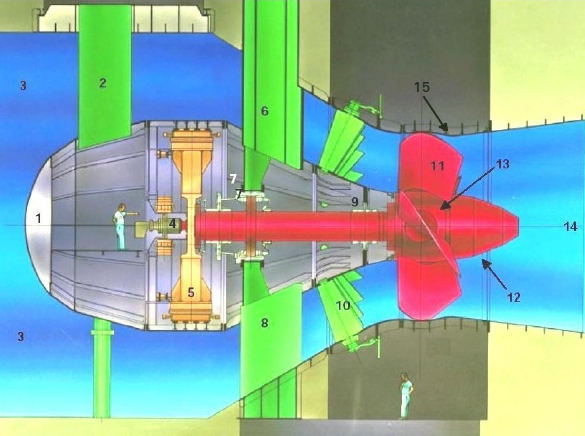
\includegraphics[width=\columnwidth]{figs/intro/bulb_turbine2}
	\caption{Ilustração de uma turbina do tipo bulbo.}
	\label{fig::bulb_turbine}
\end{figure}

\begin{center}
\begin{tabular}{  c | c  }
  \hline
  \textbf{Número} & \textbf{Componente} \\ \hline
  1 & Nariz do bulbo \\ \hline
  2 & Tubo de acesso ao gerador  \\ \hline
  3 & Câmara de adução  \\ \hline
  4 & Cabeçote Kaplan  \\ \hline
  5 & Gerador Síncrono  \\ \hline
  6 e 8 & Estrutura de sustentação \\ \hline
  6 & Tubo de acesso à turbina \\ \hline
  7 e 9 & Mancais Combinado e Guia \\ \hline
  10 & Distribuidor \\ \hline
  11 & Pás do Rotor \\ \hline
  12 & Cone ou Ogiva \\ \hline
  13 & Cubo \\ \hline
  14 & Tubo de sucção/descarga \\ \hline
  15 & Aro Câmara \\
  \hline
\end{tabular}
\captionof{table}{Componentes principais de uma turbina tipo bulbo}
%\caption{Componentes principais de uma turbina tipo bulbo}
\label{tab::bulb_turbine}
\end{center}



Atualmente, caso seja necessário algum reparo ou inspeção na turbina, é necessário que se interrompa o fluxo de água e que 
toda a água em seu interior seja drenada. Para manutenção do rotor, existe uma escotilha de acesso de diâmetro limitado. Entretanto, caso deseje-se realizar 
a metalização de pás já instaladas, utilizando-se os processos atuais, é
necessária a retirada de todo o aro câmara, desmontagem completa do rotor e logística de transporte das pás até o local
onde a metalização será realizada. Essa operação, caso necessite ser realizada, demandaria a mobilização
de diversas equipes de manutenção, operação de pórtico rolante e transporte,
além de impossibilitar a utilização da turbina durante várias semanas.
No contexto da solução proposta, os pontos de interesse da turbina são:

\begin{itemize}
  \item Hélice e pás;
  \item Aro Câmara e regiões adjacentes;
  \item Escotilhas de acesso;
  \item Tubo de Sucção;
  \item Infraestrutura disponível
\end{itemize} 

\subsubsection{Hélice e pás}
 
O rotor ou hélice da turbina é constituído do cubo, as pás e o cone. 
Nas turbinas da usina de Jirau, cada pá mede, aproximadamente, 2,5m de altura e
3m de largura. A partir do interior da turbina, todas as superfícies da pá são
alcançáveis, com exceção da borda e do lip da pá. O único ponto de acesso à
essa regiâo é por meio da escotilha superior de acesso. A figura
\ref{fig::blade_rijeza} exemplifica uma pá do rotor presente na usina de Jirau recém metalizada no galpão da Rijeza.

\begin{figure}[h!]	
	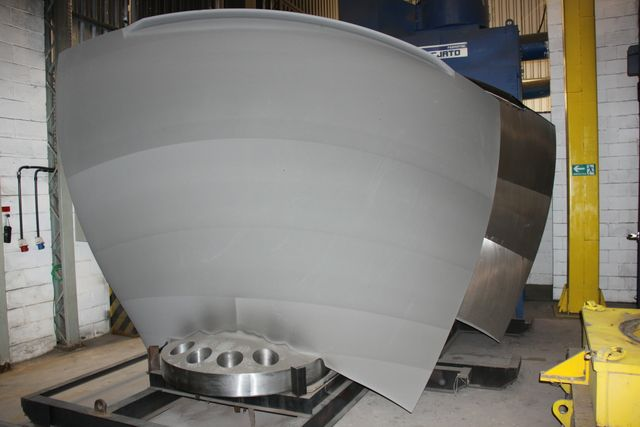
\includegraphics[width=\columnwidth]{figs/viagem/2015_04_28/Rijeza/img_4887}
	\caption{Pá do rotor recém metalizada.}
	\label{fig::blade_rijeza}
\end{figure}

A angulação de cada pá em relação ao fluxo d'água pode ser alterado em 29$^o$,
14.5$^o$ para cada lado a partir da posição inicial, não havendo sobreposição
entre as pás, como ilustrado na figura \ref{fig::blades_angle}.
Essa angulação pode ser explorada para otimizar o espaço de trabalho necessário
para o processamento da pá e também influencia o acesso à região
entre o distribuidor e o rotor, uma vez que não existe acesso pela montante da
turbina. Entretanto, vale observar que esta angulação não pode ser alterada
manualmente e só pode ser realizada uma vez, antes do desligamento da turbina. A
posição do rotor também pode ser manualmente alterada, possibilitando que o mesmo seja girado em ambas as direções e sem limite de revoluções. Entretanto, essa operação é uma tarefa imprecisa e envolve um certo risco às pessoas que a realizam. Sendo
assim, a solução proposta deve otimizar o número de rotações necessárias para o processamento de todas as pás.

\begin{figure}[h!]	
	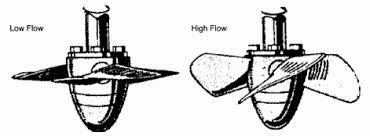
\includegraphics[width=\columnwidth]{figs/intro/blades_angle}
	\caption{Exemplo de limites de rotação das pás do rotor.}
	\label{fig::blades_angle}
\end{figure}

\subsubsection{Aro Câmara e regiões adjacentes}

O aro câmara, assim como o a região próxima ao distribuidor e também ao tubo de
sucção possuem superfícies metálicas. Essa característica possibilita a
exploração de soluções de fixação magnética.

Somente a região compreendida pelo aro câmara é plana e tendo como agravante a presença do distribuidor na região à 
montante ao rotor. É necessário que a inclinação presente nessas superfícies seja contabilizada e uma solução eficiente 
de apoio ou plano elevado seja desenvolvida caso haja necessidade de fixação de alguma parte do sistema. Atualmente todo 
o trabalho é realizado por meio da montagem de andaimes ancorados por cordas. A
figura \ref{fig::andaime} ilustra uma estrutura utilizada no modo de inspeção e
manutenção atuais.

\begin{figure}[h!]	
	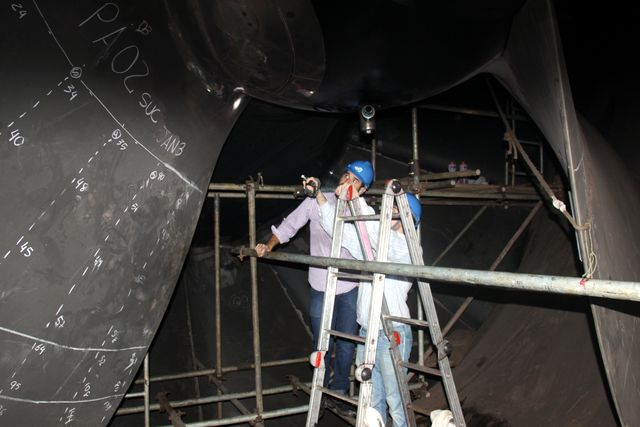
\includegraphics[width=\columnwidth]{figs/viagem/2015_04_28/UG/img_4969}
	\caption{Andaime montado no interior da turbina e ancorado por cordas}
	\label{fig::andaime}
\end{figure}

 
\subsubsection{Escotilhas de acesso}
O acesso à turbina se dá por duas escotilhas, uma inferior, localizada no ínicio do tubo de sucção 
próxima ao aro câmara e outra superior, localizada na parte superior do aro câmara.

A escotilha inferior é o acesso utilizado para a entrada de pessoas na turbina e todo 
material utilizado para reparos é transportado através dessa escotilha. Na usina de Jirau existem dois 
tipos de escotilha de acesso inferior, sendo a menor delas possuindo 80cm de diâmetro. 

A escotilha superior é utilizada, principalmente, para a inspeção visual do
estado dos Lips das pás.
O diâmetro do acesso superior é de aproximadamente $35.7cm$, limitando as
dimensões dos equipamentos que podem ser transportados através da escotilha. As figuras \ref{fig::esc_sup_ext} e
\ref{fig::esc_sup_int} ilustram o acesso à escotilha superior pelo exterior ao
aro câmara e a visão pelo interior da turbina,
respectivamente.

\begin{figure}[h!]	
	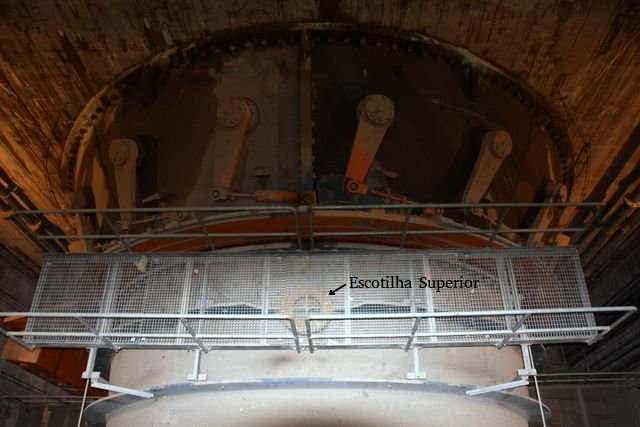
\includegraphics[width=\columnwidth]{figs/viagem/2015_04_28/UG/img_4979_mod}
	\caption{Vista da escotilha superior pelo exterior do aro câmara}
	\label{fig::esc_sup_ext}
\end{figure}

\begin{figure}[h!]	
	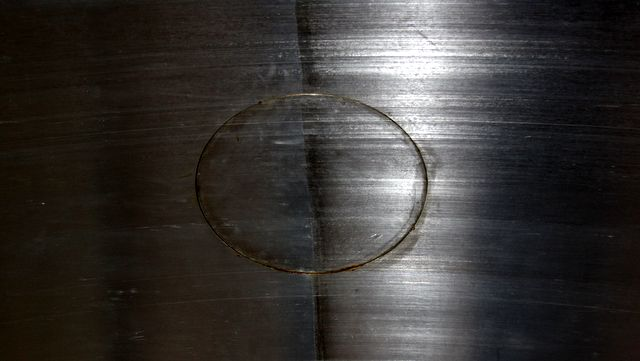
\includegraphics[width=\columnwidth]{figs/viagem/2015_04_28/UG/img_4982}
	\caption{Vista da escotilha superior pelo interior do aro câmara}
	\label{fig::esc_sup_int}
\end{figure}

\subsubsection{Tubo de sucção}

Ao final do tubo de descarga está localizado o vão dos stoplogs 
de jusante ou da comporta vagão e, em seguida, o leito do rio. Caso os stoplogs 
não estejam inseridos, existe um vão de, pelo menos, 10 m de largura. Porém, não
é válida a utilização deste vão como acesso à turbina, pois há grande fluxo de
água devido à abertura do distribuidor. O distribuidor não é fechado
imediatamente por questões ambientais, já que este é o escoamento de peixes.

%criando assim
%um acesso extra para um sistema submarino. A figura \ref{fig::tubo_suc}
%exemplifica a magnitude do tamanho do acesso, deixando claro que o limitante de
%tamanho do sistema para a utilização desse acesso é o vão de entrada do
% stoplog, ilustrado na figura \ref{fig::stoplog}. Outra alternativa é utilizar um
%guindaste e submergir o sistema pelo próprio rio, entretanto o sistema ficaria
%sujeito as condições do ambiente.

\begin{figure}[H]	
	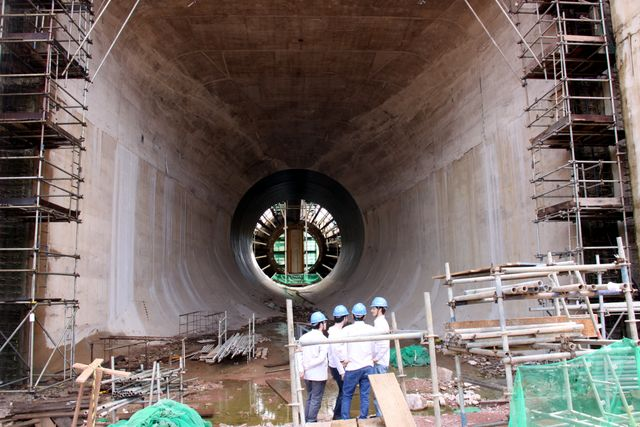
\includegraphics[width=\columnwidth]{figs/viagem/2015_04_30/Vao/img_5086}
	\caption{Abertura do tubo de sucção para o leito do rio, em fase de
	construção.}
	\label{fig::tubo_suc}
\end{figure}

\subsubsection{Infraestrutura disponível}
É importante ressaltar a infraestrutura dísponível para o desenvolvimento da solução. 
Após secar a turbina, é possível a disponibilização de energia elétrica e ar
comprimo em seu interior, ambos importantes para o processo de metalização. Outro fator 
importante é a presença de um pórtico rolante que tem acesso até o andar diretamente 
inferior ao aro câmara, posicionando todo o equipamento necessário nas proximidades 
da escotilha de acesso inferior. É possível também o acesso direto, por meio de pórtico, 
à escotilha superior.

\begin{figure}[h!]	
	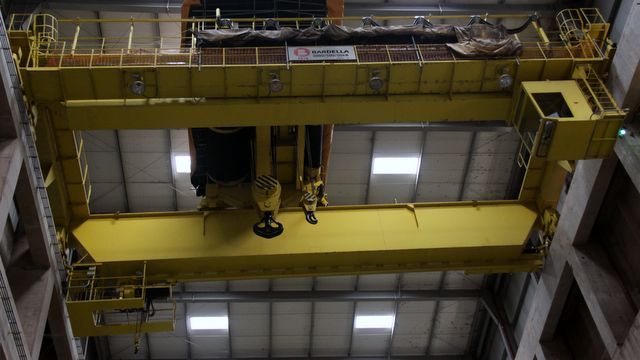
\includegraphics[width=\columnwidth]{figs/viagem/2015_04_28/UG/img_4989}
	\caption{Pórtico rolante com acesso ao exterior do aro câmara}
	\label{fig::portico}
\end{figure}


O ambiente pode ser resumidamente caracterizado pelas dimensões das pás,
elemento a ser processado; características do aro câmara, estrutura que limita o
espaço de trabalho do robô; e pelos acessos nos quais o sistema terá que
utilizar.

\begin{itemize}
  \item \textbf{Pás do rotor} - Material aço inox 420. Dimensões 2.5 x 2.5 m de superfície;
  \item \textbf{Aro Câmara} - estrutura cilíndrica com raio de 3.95 m e
  superfície metálica;
  \item \textbf{Acessos}: 
  	\begin{itemize}
    	\item Escotilha superior - 35 cm de diâmetro;
  		\item Escotilha inferior - 80 cm de diâmetro;
  		\item Tubo de descarga - 20 x 20 m, porém acessado pelo rio. 
  	\end{itemize}
\end{itemize}







\subsection{Descrição das tarefas do robô}
\label{desc_taref}
Esta subseção descreve as tarefas básicas do robô para o revestimento de
turbinas \textit{in situ}. Em linhas gerais, o robô a ser desenvolvido deve ser
capaz de realizar a tarefa de revestimento tal qual seria feita caso a pá não estivesse instalada na
tubina e de uma maneira autônoma. A pá, antes de ser submetida ao
processo de revestimento, deve estar em conformidade com o gabarito, perfil hidráulico de uma pá
intacta. Portanto, uma tarefa do robô é realizar o mapeamento do perfil
hidráulico, construir um modelo 3D e analisar imperfeições.

Em caso de deformações, causados por cavitação e abrasão, estas precisam
ser removidas manualmente ou de forma automatizada, possivelmente por
soldagem. A tarefa de soldagem pode
ser realizada por operador, manualmente, por não possuir todas as restrições
da tarefa de revestimento (velocidade, precisão, carga e etc), porém o ambiente
pode dificultar a operação de forma que a execução por um robô seja
indispensável. 

Após as pás estarem de acordo com o gabarito, faz-se a
identificação do desgaste do revestimento, medindo sua espessura em pontos
pontos específicos sobre a superfície da pá. Manualmente esse
processo é realizado eficientemente em 10 min, justificando a não necessidade de
esta ser uma tarefa do robô. 

Em caso de necessidade de aplicação
de novo revestimento, é necessária a remoção do revestimento antigo por
jateamento, a fim de deixar a superfície rugosa e aumentar sua aderência. A
tarefa de jateamento pode ser realizada pelo robô, ou manualmente
com ajuda de andaimes internos ao ambiente do aro câmara. Como ambos os lados da pá são revestidos, o
jateamento deve ser realizado em ambos os lados. Vale ressaltar que, em teoria,
pode-se aplicar revestimento por metalização sem retirar o último revestimento,
porém esse processo ainda se encontra em fase de estudos na Rijeza.
%Segue-se o exemplo de empresas de aviação, onde existe a
%prática de retirar todo o revestimento antigo antes de aplicar o novo.

Por fim, o robô deverá aplicar o revestimento como
forma de prevenir o dano causado pelos fenômenos abrasivos. O robô projetado
para fazer o revestimento precisa preencher todos os requisitos discutidos na
subseção~\ref{sec::desc_hvof} e ser adaptável ao ambiente, cujos as restrições
são discutidos na subseção~\ref{sec::desc_contex}. 

Das tarefas a serem relizadas, são destacadas as seguintes:
Tarefas que podem ser executadas manualmente:
\begin{itemize}
  \item Inspeção e análise de danos na pá, tanto para reparo quanto para
  revestimento.
  \item Reparo.
  \item Montagem do sistema.
  \item Jateamento da superfície.
\end{itemize}

Tarefas que poderão ser executadas pelo robô:
\begin{itemize}
  \item Modelar o perfil hidráulico.
  \item Calibração.
  \item Jateamento.
  \item Reparo (soldagem e esmerilhamento).
  \item Revestimento por metalização.
\end{itemize}




\section{Estado da arte}\label{sec:sota}
 
O estudo do estado da arte de robôs para a realização de HVOF em pás de turbinas
hidráulicas contempla os sistemas que atendem a alguns dos requisitos: operar
em ambientes de alta periculosidade; capacidade de carga para os dispositivos HVOF;
manipular a pistola HVOF com velocidade de $0.67 m/s$; precisão de 5mm; ter
área de trabalho de 2.5 m x 2.5 m; e operar sob superfícies 3D de geometria
complexa. As soluções foram divididas em subseções de acordo com as tecnologias
de fixação dos robôs.


 
\subsection{Robôs sobre trilhos}
%TODO características gerais do robo: fixação,
% sensores, sistema HVOF e etc
% aplicação,
% vantagens e desvantagens

%oq sao e motivaçaõ
%teconologias de fixaçaõ
%robos
%vantagems/desvantagens

Na indústria, a automatização de processos de \textit{hard coating},é
normalmente realizada com a utilização de manipuladores robóticos. Esse tipo de
robô proporciona uma versatilidade operações, uma vez que podem ser
reprogramados para realizar tarefas repetidamente com alta precisão. O espaço de
trabalho de um braço robótico é dependente do numero de juntas presentes no
robô, rotacionais ou prismáticas, e pelo tamanho de cada elo. As juntas
determinam os graus de liberdade e mobilidade que um manipulador possuí,
enquanto o tamanho dos elos influenciária no alcane máximo do robô.

Os processos de manunteção de turbinas, como o \textit{hard coating}, exigem a
realização trajetórias complexas, o que siginifica a necessidade de várias
juntas, e o tamanho das pás da turbina exigem que o manipulador tenha um alcance
máximo pelo menos maior que a maior dimensão da pá. Portanto, os manipuladores
robóticos utilizados para esse tipo de aplicação são, geralmente, robôs
industrias que pesam centenas de quilos, com mais de 2 metros de alcance máximo
e necessitam de uma fixação que garantam que o manipulador não irá se movimentar
ao realizar suas tarefas programadas. 

Para a automatização de um processo de manutenção \textit{in-situ} é
necessário, porém, que o sistema projetado seja compacto, de fácil instalação, e
que nâo exija alterações estruturais permanentes para a sua utilização. Um
manipulador robótico convencional que necessite de um espaço de trabalho
suficiente para executar tarafas em toda a superfície da pá de uma turbina se
torna, então, inviável. 

Uma estratégia para reduzir o tamanho e peso de um manipulador robótico é
torná-lo móvel. Isso pode ser alcançado com a introdução de mais uma junta
prismática acoplada a um trilho, possibilitando que o manipulador estenda seu
espaço de trabalho por toda a extensão do trilho.

Na literatura foram encontradas duas soluções para aplicações de manutenção e
inspeção, como solda. As aplicações diferem principalmente na estratégia de
fixação do trilho. O Roboturb \cite{roboturb} realiza a fixação diretamente na
pá do rotor, enquanto o robô Scompi \cite{scompi} utiliza uma fixação exterior 



\subsection{Robôs escaladores}
%TODO características gerais do robo: fixação,
% sensores, sistema HVOF e etc
% aplicação,
% vantagens e desvantagens
Robôs escaladores são sistemas capazes de sustentar seu próprio peso contra a
gravidade, movendo-se em simples ou complexas estruturas geométricas, como
paredes, tetos e telhados, palhetas de turbinas e plantas nucleares.
Essa classe de robôs oferece eficiência operacional em ambientes
de alta periculosidade, sendo utilizados visando saúde e segurança dos
trabalhadores, como em inspeção e limpeza de arranha-céus, diagnóstico de
tanques de armazenamento em plantas nucleares, solda e manutenção de cascos de
navios e palhetas de turbinas \cite{clawar}.

Os grandes desafios nos projetos de sistemas escaladores são mobilidade e
aderência, além de consumo de energia, capacidade de carga e peso. Em
\cite{modular}e \cite{climbsurv}, os robôs escaladores são divididos em tipos de locomoção:
pernas, como andador, utilizando segmentos deslizantes, rodas, esteiras, avanço
pendurado por braços, por cabos e biomimética; e categorias de adesão: sucção ou
pneumática, magnética, eletrostática, química, preensão e híbrida.

No caso específico deste estudo da arte, destacam-se os robôs escaladores com as
seguintes aplicações:

\begin{itemize}
  \item \emph{Construção de navios e turbinas}: RRX3 para soldagem
  \citep{rrx3}, \emph{Climbing Robot for Grit Blasting} para limpeza
  \citep{crgb} e ICM Robot para inspeção \citep{icm};
  \item \emph{Construção industrial}: ROMA II \citep{roma} e
  CROMSCI \citep{CROMSCI}, ambos para inspeção; 
 \item \emph{Planta petroquímica}: ROBICEN \citep{robicen} e
  TRIPILLAR \citep{tripillar}, ambos para inspeção.  
\end{itemize}

O RRX3 é um robô para a soldagem de casco de navios. Possui adesão por
preensão, locomoção transversal utilizando segmentos deslizantes e locomoção
longitudinal por rodas. Possui um manipulador de 1.5 m com três juntas
prismáticas e três juntas de revolução (3P3R) para a operação de soldagem. Suas
principais vantagens e desvantagens em relação à aplicação HVOF são:

\textbf{Vantagens:}
\begin{itemize}
  \item Base com capacidade de carga 120 kg;
  \item Manipulador com capacidade de carga 5 kg;
  \item Manipulador de precisão milimétrica;
  \item Robô robusto que trabalha com instrumento de alta temperatura (solda);
\end{itemize}

\textbf{Desvantagens:}
\begin{itemize}
  \item Locomoção restrita impede utilização em estruturas geométricas
  complexas;
  \item Manipulador não possui alcance suficiente para a aplicação fim;
  \item Manipulador com efetuador de baixa velocidade;
\end{itemize}

O \emph{Climbing robot for Grit Blasting} é um robô para jateamento abrasivo em
navios. O robô utiliza duas plataformas deslizantes com sistema de adesão por
ímã magnético. Os módulos apresentam movimentação relativa entre si e pode rotar
para compensar as curvaturas do casco do navio ou desviar de objetos. 

\textbf{Vantagens:}
\begin{itemize}
  \item Base com capacidade de carga de sistema abrasivo semelhante ao HVOF;
  \item Base com locomoção de precisão milimétrica;
\end{itemize}

\textbf{Desvantagens:}
\begin{itemize}
  \item Locomoção ampla, porém não aplicável às estruturas geométricas
  complexas. A curvatura do casco é simples quando comparada à pá da turbina;
  \item Não possui manipulador, logo o sistema deve percorrer todo o
  casco;
  \item A instalação de um manipulador prejudica a estabilidade do sistema;
\end{itemize}

\emph{The Climber}, ICM Robotics, é um robô para inspeção de turbinas eólicas,
remoção de revestimento, limpeza de superfície, e aplicação de revestimento.
Possui adesão pneumática (sucção) e locomoção por esteiras. 

\textbf{Vantagens:}
\begin{itemize}
  \item Base com capacidade de carga de 25 kg;
  \item Base com locomoção de precisão milimétrica;
  \item Manipulador para revestimento HVOF pode ser acoplado à base; 
\end{itemize}

\textbf{Desvantagens:}
\begin{itemize}
  \item Manipulador com baixo alcance;
  \item Manipulador com efetuador de baixa velocidade;;
  \item Locomoção apresenta restrição a certas curvaturas devido às esteiras;
\end{itemize}

O ROMA II, Universidade Carlos II de Madrid, é um robô para inspeção de
ambientes complexos. A sua tecnologia de adesão é pneumática (sucção) e
locomove-se como uma lagarta (biomimética). Sua movimentação e planejamento de
trajetória são realizados de maneira ótima de forma a garantir estabilidade e
evitar obstáculos. 

\textbf{Vantagens:}
\begin{itemize}
  \item Base com grande capacidade de carga;
  \item Base com locomoção de grande precisão;
  \item Movimenta-se em ambientes de grande complexidade geométrica; 
\end{itemize}

\textbf{Desvantagens:}
\begin{itemize}
  \item Não possui manipulador para aplicação HVOF;
  \item A instalação de um manipulador irá desequilibrar o sistema,
  principalmente durante a locomoção;
\end{itemize}


CROMSCI, Kaiserslautern University of Technology, é um robô autônomo para
inspeção de grandes paredes de concreto, como pilares de pontes, barragens. Seu
sistema de adesão é composto por sete câmaras de vácuo (sucção), com um sistema
de controle por válvulas e sensores de pressão para reagir rapidamaente a
condições adversas. Locomove-se com rodas omnidirecionais para locomoção.

\textbf{Vantagens:}
\begin{itemize}
  \item Base com locomoção de precisão milimétrica; 
\end{itemize}

\textbf{Desvantagens:}
\begin{itemize}
  \item Manipulador com alcance de 80 cm;
  \item Manipulador com efetuador de baixa velocidade;
  \item Protótipo ainda com pouca capacidade de carga;
\end{itemize}

Planta petroquímica: ROBICEN

TRIPILLAR, École polytechnique fédérale de Lausanne, é um robô escalador de
pequeno porte (96 x 46 x 64 mm) desenvolvido para a inspeção de plantas
petroquímicas. Utiliza um sistema como pernas de lagarta magnéticas em um
formato triangular. Locomove-sepor esteiras.

\textbf{Vantagens:}
\begin{itemize}
  \item Base com locomoção de precisão milimétrica;
  \item Sistema robusto;
  \item Controle simples;
  \item Pequenas dimensões; 
\end{itemize}

\textbf{Desvantagens:}
\begin{itemize}
  \item Não foi testado em estruturas de grande complexidade geométrica; 
  \item Não apresenta manipulador;
  \item Protótipo ainda com pouca capacidade de carga;
\end{itemize}
   

\subsection{Robôs Cabeados}
% 1 OQ SAO, MODTIVACAO
% 2 TECNOLOGIA DE FIXACAO
% 3 NOSSOS ROBOS
% Vantagens e desvantagens
%TODO características gerais do robo: fixação,
% sensores, sistema HVOF e etc
% aplicação,
% vantagens e desvantagens

São classificados como robôs cabeados quaisquer sistemas robôticos que façam
uso de um conjunto de cabos e/ou cordas para auxiliar ou mesmo garantir seu
posicionamento adequado na sua região de trabalho. Sendo assim, robôs cabeados
podem possuir outros métodos de fixação em conjunto com seu cabeamento.

A idéia do uso de um sistema de cabos surge naturalmente, quando o deslocamento
se mostra majoriamente restrito a um plano vertical e não há exigência de
grandes velocidades de deslocamento, como forma de reduzir o preso e melhorar o
desempenho de um braço mecânico de mesmo alcance, ou diminuir a complexidade e
a força de aderência necessária para um \textit{crawler}.



\subsection{Manipulador com base esférica}
%TODO características gerais do robo: fixação,
% sensores, sistema HVOF e etc
% aplicação,
% vantagens e desvantagens
Um projeto de pesquisa e desenvolvimento foi apresentado em
\cite{motta2010prototype} com o objetivo de propor metodologia, simulação e
os passos para construção de um sistema robótico para recuperar danos materiais
em pás de turbinas hidráulicas gerados devido à cavitação. O sistema robótico faz
reparo utilizando a tecnologia de soldagem a arco elétrico, antes realizada
manualmente em ambientes de alta periculosidade com temperaturas que variam
entre $40^o C$ e $99^o C$ em operações que duram em torno de 10 horas.

O robô deve atender aos seguintes requisitos:
\begin{itemize}
  \item Capacidade de operar em qualquer posição: horizontal, vertical,
  invertida;
  \item Pouco peso para portabilidade e fixação às pás;
  \item Rigidez à deflexão: carga no punho do manipulador ocorre em qualquer
  direção e extensão;
  \item Grande precisão na mobilidade;
  \item Disponibilidade de peças no mercado;
  \item Controle com interface de usuário;
  \item Grande área de trabalho;
  \item Facilidade de adesão às pás de turbinas hidráulicas.
\end{itemize}

A solução para o sistema robótico apresenta topologia esférica, como pode ser
visto na figura~\ref{fig:esferico} e características:

\begin{figure}[ht]
\centering
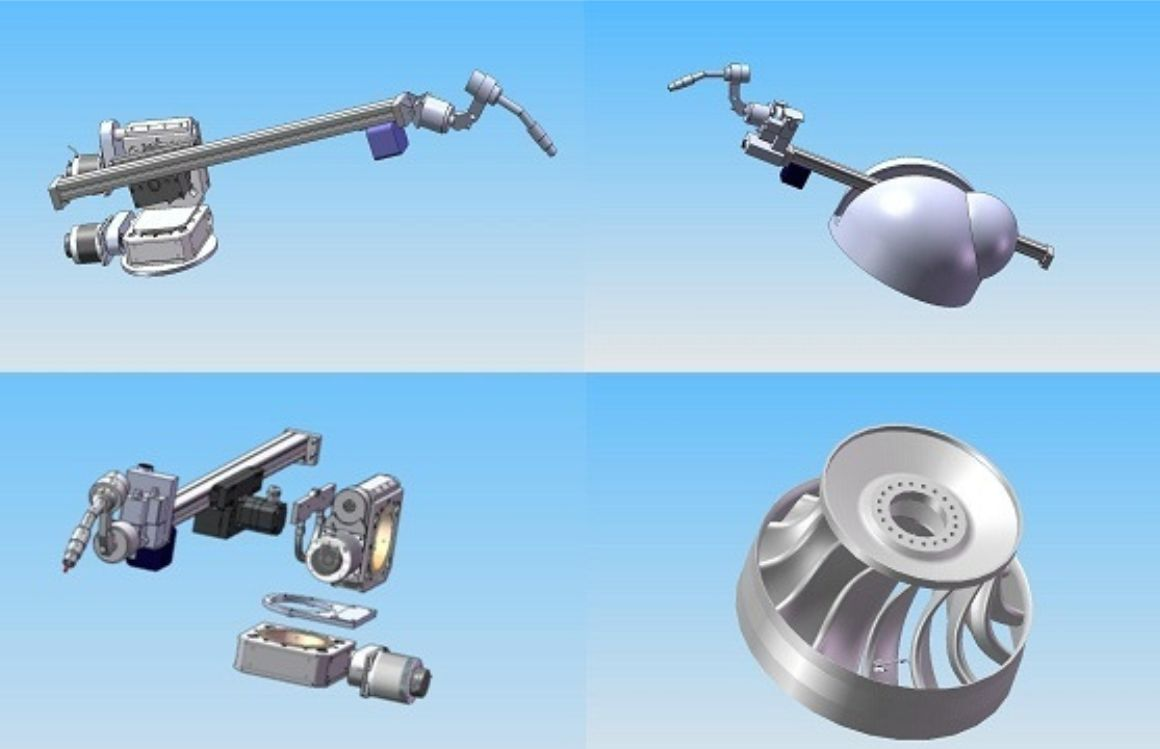
\includegraphics[width=8.4cm]{figs/esferico/esferico.jpg}
\caption{Ilustração do projeto do manipulador com base esférica.}
\label{fig:esferico}
\end{figure}

\begin{itemize}
  \item Três (3) graus de liberdade no manipulador (2R1P) e dois graus de
  liberdade no punho (2R);
  \item Mapeamento de superfície 3D com laser;
  \item Eletrônica embarcada;
  \item Soldagem por arco elétrico;
  \item Fixação nas pás por dispositivos magnéticos ou de sucção;
  \item Baixo custo;
  \item Área de trabalho em forma de anel com 2.5 m e 60 cm de altura;
  \item Peso 30 kg e dimensões 30 x 25 x 100 cm;
  \item Robô com manipulador autônomo;
\end{itemize}

O sistema robótico de manipulador com base esférica apresenta solução compatível
para a aplicação de HVOF em pás de turbinas hidráulicas, já que sua aplicação
original é soldagem das pás, semelhante ao desafio deste artigo. Todas as suas
características são vantagens e aplicam-se à solução de um sistema para HVOF.
Há, porém, desafios particulares na metalização das pás e que são desvantagens
da solução:

\begin{itemize}
  \item A metalização deve ser realizada em toda a pá. Portanto, o sistema
  deverá ser manualmente trocado de posição, pelo menos 4 vezes (duas posições
  para a frente e duas posições para a região de trás). E deve ser trocado de pá
  em pá;
  \item O efetuador deve percorrer a pá com grande velocidade, como exige o
  processo de metalização.
\end{itemize}

%TODO concluir sota

\section{Projeto de robô autônomo para HVOF}\label{sec:projeto}

% TODO soluções e dificuldades comuns
O projeto de robôs autônomos para HVOF em pás de turbinas hidráulicas contempla
as soluções que atendem a \textbf{todos} os requisitos da aplicação. Dessa
forma, serão idealizados robôs com a fusão das tecnologias expostas na
seção~\ref{sota}.
 
\subsection{Acesso pela escotilha de dimensão pequena}
%TODO Elael: prós e contras do acesso, soluções: manipuladores
% industriais, manipuladores customizados, trilhos. Incluir figuras do
% posicionamento das pás e cálculos do tamanho mínimo do manipulador

\subsection{Acesso pela escotilha de dimensão grande}
Soluções que utilizem o acesso pela escotilha inferior, de dimensão maior,
apresentam as seguintes vantagens e desvantagens:

\textbf{Vantagens}:
\begin{itemize}
  \item Abertura maior para passagem de robôs pequenos montados ou um robô
  grande desmontado;
  \item Toda operação é realizada a seco;
  \item O acesso é livre;
  \item Este acesso já é usado pelos operadores para manutenção da turbina;
\end{itemize}

\textbf{Desvantagens}
\begin{itemize}
  \item Não é suficientemente grande para entrada de robôs de grande
  porte montados;
  \item Infraestrutura de transporte e complexa logística ao acesso por
  andaimes e talha;
  \item Dificuldade de movimentação e posicionamento do robô no aro câmara
  devido ao piso escorregadio e inclinado. Pode haver a necessidade de montagem
  de um plano horizontal; 
\end{itemize}

O acesso pela escotilha inferior apresenta, como todos os outros
acessos, um desafio logístico e o desafio comum do processo de metalização. O
acesso à escotilha é realizado por um buraco de 80 mm de diâmetro e 4 m acima do
solo, logo os equipamentos são transportados por uma talha operada manualmente,
instalada dentro do aro câmara, em andaimes. O solo é escorregadio e, devido à
forma cilíndrica do aro câmara, curvilíneo e inclinado.

Dessa forma, as soluções foram focadas em robôs de médio porte, peso reduzido
devido ao transporte e à necessidade de movimentação e posicionamento do robô
(trajeto escotilha à pá) e modular, quando possível.

As soluções foram divididas em subseções de acordo com a fixação: robôs móveis
que se locomovem em trilhos, manipuladores industriais com base fixa e sistema
fixo à pá. 
%obs.:
%Colocar o robô entre as pás para aplicar revestimento de duas pás com uma
% instalação exige que o robô seja desmontado toda vez que a turbina for girada.
%Isso é ruim, pois após primeira aplicação a área fica de risco. Esta solução
%exige 5 movimentos no robô e 6 movimentos na turbina.

%A solução em que o robô fica atrás ou à frente exige que o robô seja
%movimentado apenas 2 vezes e a turbina fará 8 movimentos (duas voltas).

%TODO revisar todos os projetos sabendo as respostas
\subsubsection{Projeto de robôs em trilhos}\label{proj_rail}
 % attach a rail to the blade and move it manually
 
 % attach a rail one the nose and ground, 1D movement and move the blade to
A utlização de um manipulador robótico sobre trilhos satisfaz todos os
requisitos para a realização de um processo de inspeção e metalização utilizando a técnica HVOF. O desenvolvimento
de um sistema compacto para o transporte através do acesso pela escotilha
inferior e sua instalação no aro câmara da turbina são possíveis, pois as
dimensões do manipulador podem ser reduzidas por meio da
mobilidade extra proporcionada pela introdução do trilho.

No contexto da aplicação proposta, foram concebidas duas possibilidades para a
fixação do sistema de trilhos. A primeira solução consiste em um sistema
semelhante ao Roboturb, apresentado na seção \ref{sec::rail}. O sistema proposto
se trata de um manipulador robótico com fixação diretamente na própria pá da
turbina. O trilho deverá ser flexível para ser capaz de acompanhar a curvatura
da pá e possibilitar diversas opções de posicionamento. Como o material da pá
não possui alta permeabilidade magnética (Inox 420), a solução de fixação seria
por ventosas ativas e com material específico para suportar as grandes
variações de temperatura que a pá pode alcançar (temperatura ambiente a
$100^oC$ durante a metalização).

Uma abrangente pesquisa de robôs comerciais industriais de pequeno porte apontou
que há manipuladores com payload (entre 12 e 20 kg) e velocidade necessários,
sendo o LBR da Kuka o que possui melhor benefício peso/alcance, 30 Kg e 820 mm,
respectivamente. Para este manipulador, a metalização deverá ser
realizada em, pelo menos, quatro etapas com quatro trilhos diferentes e
customizados, e placas de sacrifício para evitar mau aplicação da metalização
durante as trocas de sentido na movimentação do robô.

A fixação de um trilho na pá apresenta diversas complexidades, como: a
necessidade de manualmente instalar/desinstalar o sistema trilho/robô oito vezes
em cada pá; o projeto do trilho customizado e flexível; e ventosas ativas
especiais que suportam variação de temperatura.

A alternativa para se evitar o contato com a pá consiste em um único trilho
retilíneo fixado por bases magnéticas no solo do aro câmara. Como o robô não
tem alcance de toda a pá, há, ainda, a necessidade de três posições verticais
diferentes. A pá pode ser processada em diagonal, e, neste caso, o manipulador
ficará responsável pela velocidade, posição e orientação do processo. Ou processada na
direção do trilho, e, neste caso, este ficará responsável pela velocidade e o
manipulador fará o controle de posição e orientação. Neste último, a troca de
sentido de movimento ocorrerá fora da pá, o que resulta na ausência de placas de
sacrifício. A figura~\ref{rail2} mostra o trilho externo à pá e com
processamento diagonal.

\begin{figure}[h!]
\centering
	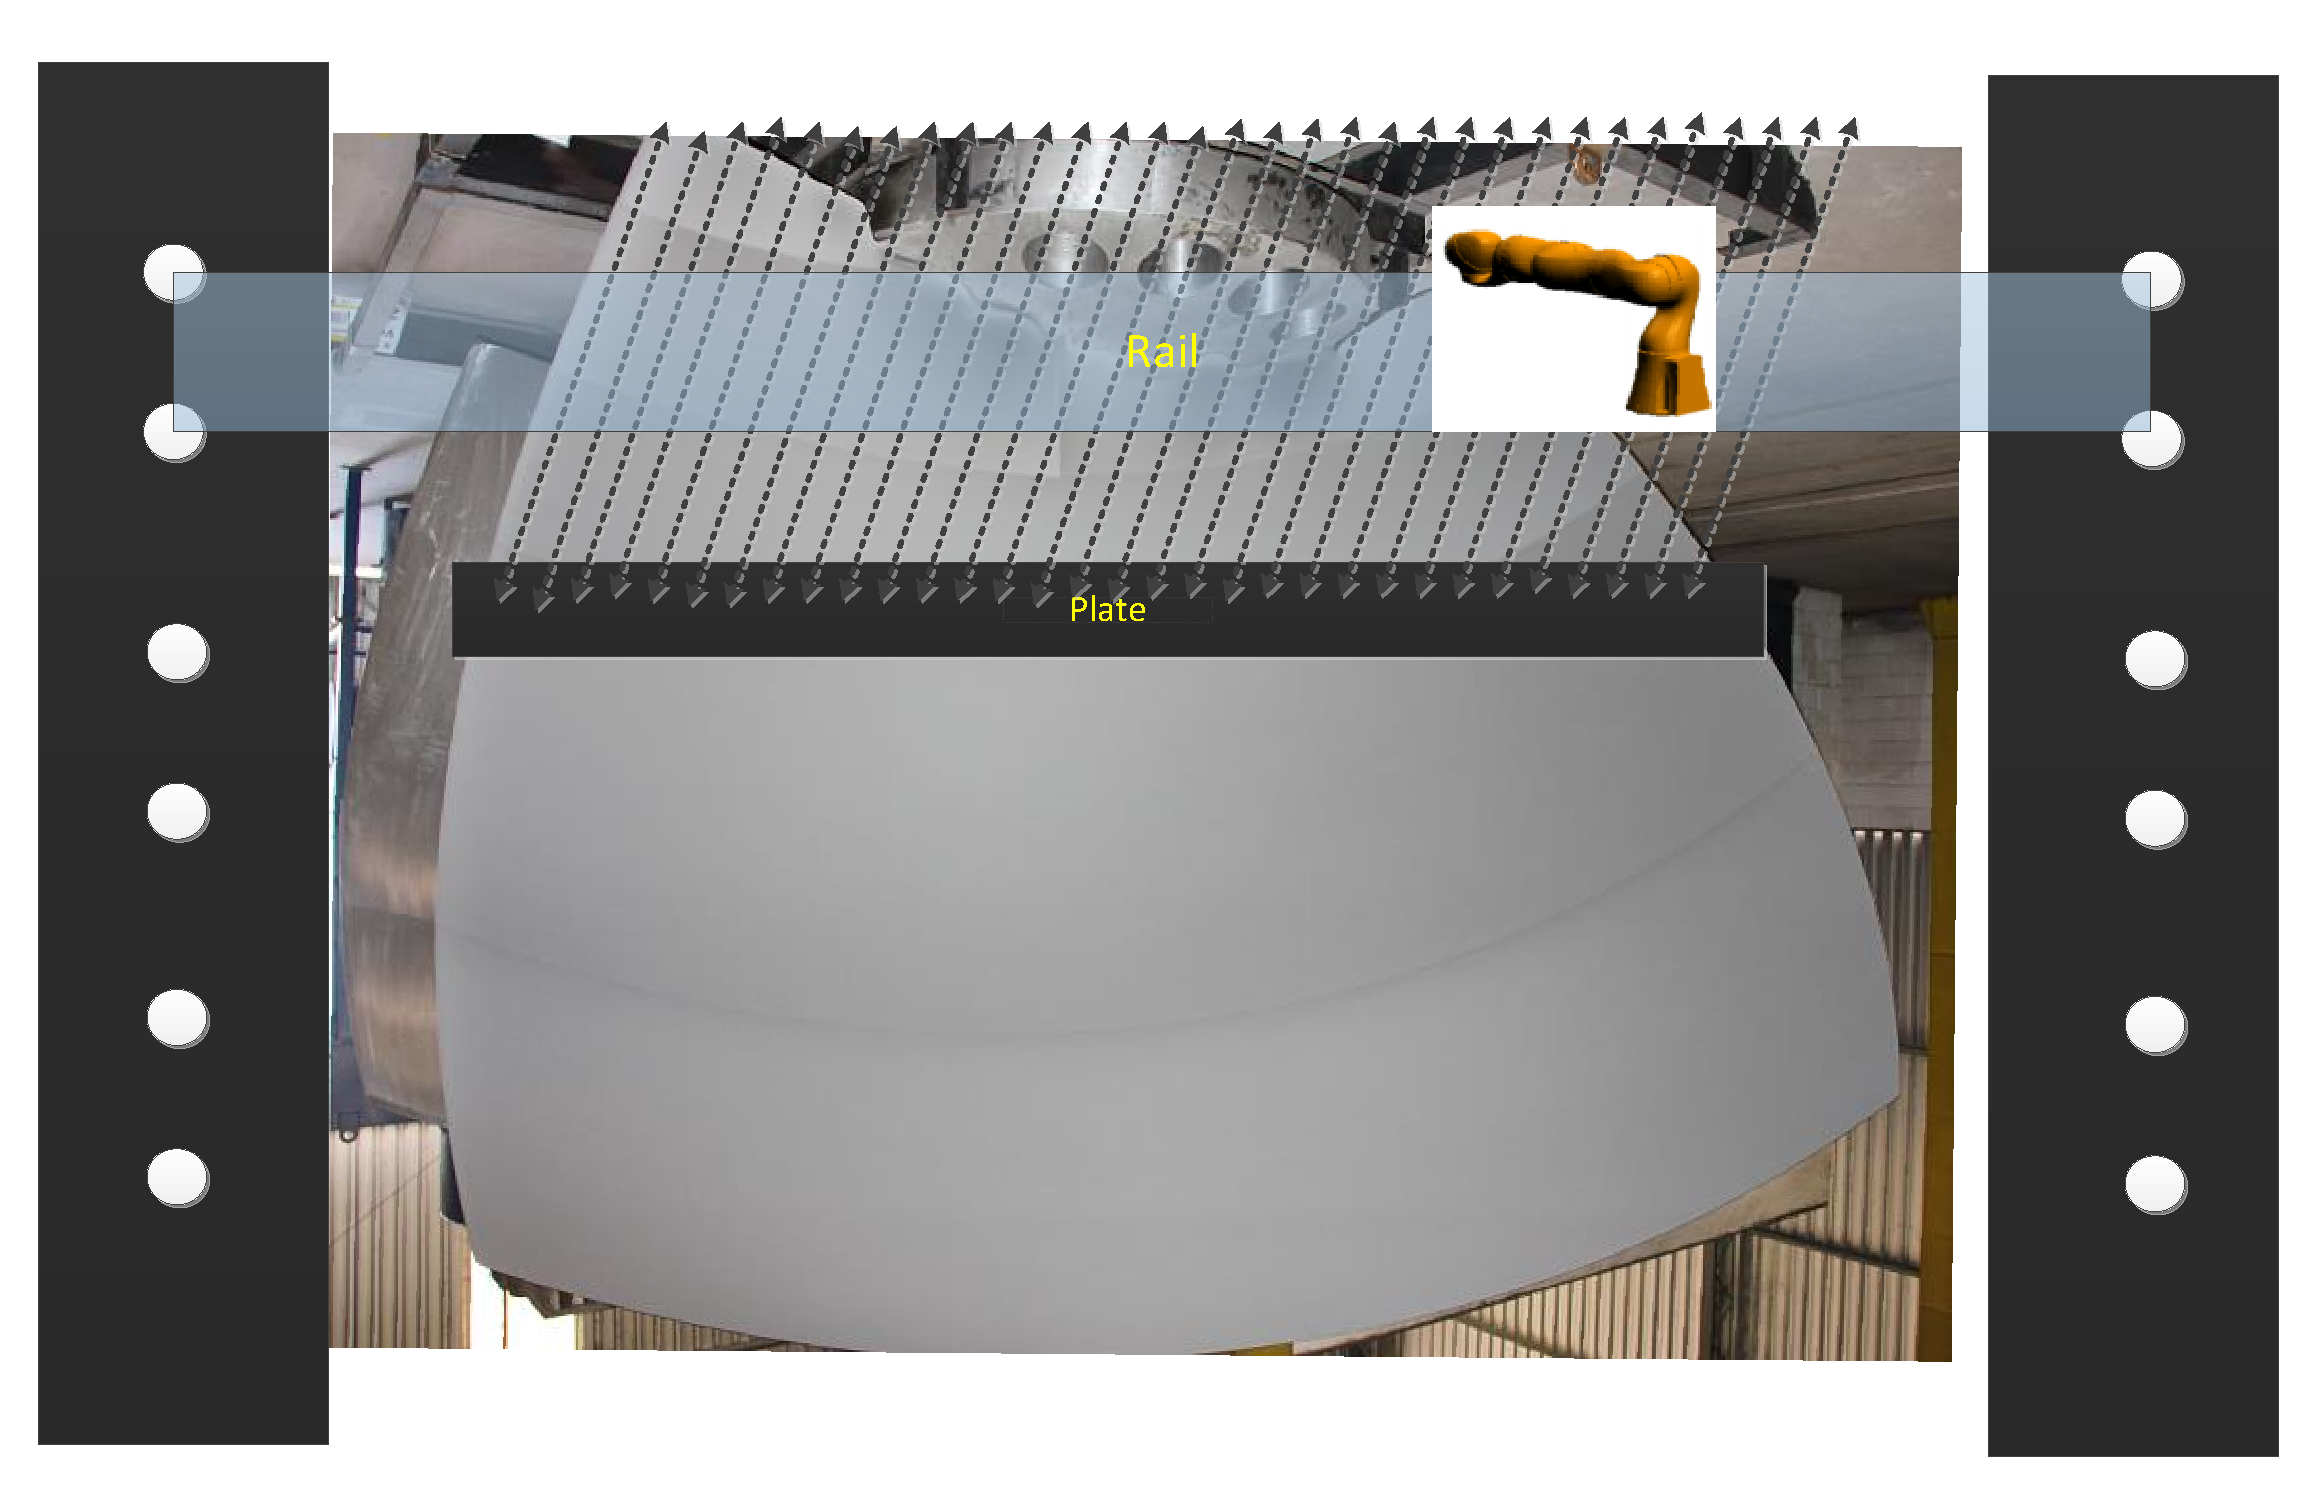
\includegraphics[width=\columnwidth]{figs/trilhos/rail2.pdf} 
	\caption{Trilho fora da pá com processamento em diagonal.}
	\label{rail2}
\end{figure}

Esse tipo de abordagem simplifica a movimentação do robô no
trilho, uma vez que o trilho seria totalmente reto, e possibilitaria a
metalização de um dos lados das quatro pás com uma única instalação de base.
Porém, mesmo nesta solução, a altura do trilho deverá ser ajustada três vezes para
cada lado de pá, e toda a estrutura deverá ser reinstalada no outro lado da
turbina para a realização do processo no outro lado das pás.

Em ambos os sistemas propostos, é necessária a implementação de um sistema de
localização do robô em relação à pá, tornando possível a geração de um
planejamento de trajetórias para o processo de metalização. O sistema de
localização pode ser concebido por sensores externos
ao robô (câmeras e outros), ou instalados no próprio manipulador/base.

\textbf{Conclusão da solução por robôs em trilhos}
A solução com trilho externo se mostrou vantajosa em comparação ao robô em
trilho customizado acoplado à pá, devido à complexidade e intervenções
manuais. Há a possibilidade de utilizar um manipulador industrial, tornando o
foco do projeto em processamento de sinais, mapeamento, localização e controle,
além da construção do trilho. Porém, a montagem da estrutura e a instalação de
todo o sistema atrás da pá podem ser custosas, sendo esta ainda uma solução
considerada complexa.
\subsection{Projeto de robôs escaladores}\label{proj_climbers}
% "scan" use succion-based mobile system (ICM climber) and place an arm on it.
% Is blade is above maximal curvature ?
% rail em movimento
Nesta subseção, consideram-se soluções para HVOF de pás de turbinas robôs
escaladores com fusão das tecnologias documentadas na
seção~\ref{sota}, subseção~\ref{sota_climbers}.

A solução mais completa, que mais atendia às especificações e possibilita
aperfeiçoamento 
\subsubsection{Projetos com manipuladores industriais fixos}\label{proj_manip}
Há diversos manipuladores robóticos industriais com as especificações
necessárias para a realização da tarefa de metalização por HVOF. As empresas
Fanuc, Motoman, ABB e KUKA fabricam manipuladores com dimensões compatíveis com o
acesso pela escotilha inferior e velocidade, precisão, e espaço de trabalho que
cumprem os requisitos para a execução do processo em todo um lado da pá, em uma
base fixa. Porém, há a necessidade de escolher a posição correta do manipulador
em relação à pá, a fim de maximizar a sua área de trabalho, no ambiente da
turbina, o que pode restringir os seus movimentos.
Como as pás podem ser giradas até um ângulo de $14.5^o$, são discutidas as ideias de posicionamento
do manipulador entre as pás, a fim de executar a operação em ambos os lados da
pá (um lado de cada pá), e o posicionamento fixo à frente da pá.

\textbf{Posicionamento entre pás}
A figura~\ref{fig::andaime} mostra o espaço entre as pás da turbina, dentro do
aro câmara. Um robô manipulador de médio porte pode ser fixado em uma base
magnética, na posição que se encontra a escada da figura~\ref{fig::andaime}.
Essa posição é vantajosa por possibilitar a execução da tarefa em duas pás
(frente de uma e verso da outra), sem desmontar ou fazer grandes alterações no
posicionamento da base do robô, diminuindo as intervenções e tempo de tarefa.

O estudo puramente geométrico demonstra que o alcance do manipulador robótico
para o processamento de ambos os lados das pás, considerando uma base fixa entre
as pás, deverá ser em torno de 5 metros. O manipulador industrial IRB5500,
desenvolvido pela ABB para pintura, possui 3 metros de alcance, porém 180 kg, o que já dificulta ou até impossibilita a
logística de movimentação e posicionamento in-situ. Não foi encontrado um robô
industrial com o alcance necessário e que tivesse as dimensões máximas da
escotilha inferior. 

A solução conceitual de posicionar um manipulador industrial entre as pás deve
avaliar, portanto, todas as configurações necessárias da base (orientações e
posições) para garantir que todo o espaço de trabalho do manipulador mais base
cubra os lados de ambas as pás. O número de configurações e o projeto
mecânico da base são extremamente necessários para a viabilização da solução,
uma vez que será possível avaliar as intervenções e complexidades. Bases
autônomas diminuem o número de intervenções e aumentam a precisção do sistema,
porém aumentam a complexidade, o custo devido ao número de sensores e atuadores
e o peso do sistema, prejudicando a logística.

\textbf{Posicionamento à frente da pá}
Posicionar de maneira fixa um manipulador com base magnética à frente da pá para
a metalização é uma solução natural, já que é semelhante à utilizada pela
empresa Rijeza atualmente. Um estudo puramente geométrico, utilizando as
dimensões da pá, mostra que o manipulador deve possuir alcance de 1.7 m e ser
posicionado a uma altura de 1.1 m em relação ao solo. Estudos de espaço de
trabalho, manipulabilidade e colisões devem ser realizados para confirmar o
estudo geométrico.

O posicionamento do sistema à frente da pá exige intervenções para rotação da
turbina e para o deslocamento do sistema para trás da pá. Em relação a um
sistema com base autônoma entre as pás, o processo parece mais custoso em
intervenções manuais e mais demorado, porém bem mais simples.

\textbf{Conclusão da solução com manipuladores industriais}
A utilização de manipuladores industriais é a mais simples dentre todas as soluções para o acesso pela escotilha inferior. Não há projeto mecânico
do manipulador, já que este será adquirido em um dos fabricantes citados. As
dificuldades mecânicas do projeto serão em relação à logística de posicionamento
e movimentação do robô dentro do aro câmara, e no desenvolvimento de uma base,
que pode ser autônoma. Além disso, o projeto fica responsável pelo controle do
manipulador, processamento de dados que envolvem o HVOF, planejamento de
trajetórias e UI.

Este projeto conceitual será uma das frentes para o estudo de viabilidade.
 
% RIWEA-like rail on which the coating system
%  place blade horizontal and use wheels, against the blade's rim,to move a rail
  % along the blade's shape
  %  two-arm solution (or one arm + magnetic attachment point) to allow reaching
  % the top of the blade from the very bottom
\subsection{Robô Bipartido}

Esse conceito é uma cadeia de dois manipuladores conectados por um ponto de
apoio capaz de fixar-se à pá. O apoio serve como forma reduzir o torque
necessário nas juntas ao reduzir a alcance necessário para cada manipulador
individualmente.

Para facilitar futuras referências nesse texto, o braço robótico que se
apoia sobre o chão será chamado de primário, manipulador que parte dele de
secundário e o ponto de apoio entre eles, capaz de fixa-se à pá, será chamado de
fixador.

 A pistola de metalização presa ao manipulador secundário deve ter
alcance sobre toda a pá da turbina. Para isso existe uma gama de pontos
necessários onde o fixador deve ser posicionado. Com esse intuito o
manipulador primário da cadeia precisa ser projetado para ter uma região de
trabalho com um alcance total sobre esses pontos. Para tal, informações precisas
sobre o formato das pás são necessárias.

Para viabilizar a solução, é necessário verificar quais são as soluções
possíveis para gerar a aderencia do fixador sobre à pá. As tecnologias mais
difundidas são por força magnética e por diferença de pressão (ventosa).
As maiores preocupações com o relação a adesão são a capacidade de carga do
método e a resistência do \textit{coating}. As soluções por magnetismo e
por ventosa afetam de maneira diferente as camadas do material ao qual se
aderem. Enquanto o magnetismo atrai ativamente o material ao qual prentende
aderir, a ventosa apenas reduz a pressão do ar na região onde ela se fixa. Ambas
as soluções possuem versões ativas e passivas, assim como uma gama de opções com
relação à capacidade de suportar carga. Logo, para essas soluções, a carga
necessária a ser suportada, o magnetismo do material, a resistência à baixa
pressão do \textit{coating} e os efeitos da atração magnética, também, sobre o
\textit{coating} são perguntas que devem ser respondidas.

O braço secundário deve ser projetado para atingir os requerimentos de
posicionamento e velocidade da pistola de metalização, porém a região sob o
fixador, certamente, não estará disponivel para receber o revestimento. Assim, a
possibilidade, ou os requisitos necessários, de mover o fixador para uma região
da pá recém metalizada deve ser vista analisada antes do robô bipartido ser
considerado uma possibilidade.

\subsection{Robô Pendurado} 


 % attach a rail to the blade and move it manually
 
 % attach a rail one the nose and ground, 1D movement and move the blade to
 

\subsection{Projeto de robôs escaladores}\label{proj_climbers}
% "scan" use succion-based mobile system (ICM climber) and place an arm on it.
% Is blade is above maximal curvature ?
% rail em movimento
Nesta subseção, consideram-se soluções para HVOF de pás de turbinas robôs
escaladores com fusão das tecnologias documentadas na
seção~\ref{sota}, subseção~\ref{sota_climbers}.

A solução mais completa, que mais atendia às especificações e possibilita
aperfeiçoamento 
 
% RIWEA-like rail on which the coating system
%  place blade horizontal and use wheels, against the blade's rim,to move a rail
  % along the blade's shape
  %  two-arm solution (or one arm + magnetic attachment point) to allow reaching
  % the top of the blade from the very bottom
\subsection{Robô Bipartido}

Esse conceito é uma cadeia de dois manipuladores conectados por um ponto de
apoio capaz de fixar-se à pá. O apoio serve como forma reduzir o torque
necessário nas juntas ao reduzir a alcance necessário para cada manipulador
individualmente.

Para facilitar futuras referências nesse texto, o braço robótico que se
apoia sobre o chão será chamado de primário, manipulador que parte dele de
secundário e o ponto de apoio entre eles, capaz de fixa-se à pá, será chamado de
fixador.

 A pistola de metalização presa ao manipulador secundário deve ter
alcance sobre toda a pá da turbina. Para isso existe uma gama de pontos
necessários onde o fixador deve ser posicionado. Com esse intuito o
manipulador primário da cadeia precisa ser projetado para ter uma região de
trabalho com um alcance total sobre esses pontos. Para tal, informações precisas
sobre o formato das pás são necessárias.

Para viabilizar a solução, é necessário verificar quais são as soluções
possíveis para gerar a aderencia do fixador sobre à pá. As tecnologias mais
difundidas são por força magnética e por diferença de pressão (ventosa).
As maiores preocupações com o relação a adesão são a capacidade de carga do
método e a resistência do \textit{coating}. As soluções por magnetismo e
por ventosa afetam de maneira diferente as camadas do material ao qual se
aderem. Enquanto o magnetismo atrai ativamente o material ao qual prentende
aderir, a ventosa apenas reduz a pressão do ar na região onde ela se fixa. Ambas
as soluções possuem versões ativas e passivas, assim como uma gama de opções com
relação à capacidade de suportar carga. Logo, para essas soluções, a carga
necessária a ser suportada, o magnetismo do material, a resistência à baixa
pressão do \textit{coating} e os efeitos da atração magnética, também, sobre o
\textit{coating} são perguntas que devem ser respondidas.

O braço secundário deve ser projetado para atingir os requerimentos de
posicionamento e velocidade da pistola de metalização, porém a região sob o
fixador, certamente, não estará disponivel para receber o revestimento. Assim, a
possibilidade, ou os requisitos necessários, de mover o fixador para uma região
da pá recém metalizada deve ser vista analisada antes do robô bipartido ser
considerado uma possibilidade.

\subsection{Robô Pendurado} 

\subsection{Acesso pela jusante}
%TODO Abelha: prós e contras do acesso, soluções, apresentar soluções de
% logística


Como última opção de acesso ao rotor existe a possibilidade de utilização do
tubo de sucção ou descarga como meio de entrada à turbina. Com o fluxo de água
parado, é possível utilizar o Rio como meio de lançamento do sistema. A
complexidade da operação para utilizar esse acesso é maior, entretanto existem
vantagens que podem tornar essa solução possível e mais atrativa.

\textbf{Vantagens}
\begin{itemize}
  \item Virtualmente nenhuma restrição de tamanho
  \item Flexibilidade de soluções
  \item Facilidade de utilização de um manipulador industrial \textit{standard}
  \item Possibilidade de implementação em outras usinas
\end{itemize}

\textbf{Desvantagens}
\begin{itemize}
  \item Complexidade de lançamento e recuperação
  \item Custo
  \item Possibilidade de correnteza
  \item Complexidade logística de transporte entre a entrada do tubo de sucção e
  o aro câmara
  \item Complexidade de prototipação
\end{itemize}

As possíveis soluções foram divididas nas etapas necessárias para a operação, ou
seja, lançamento e recuperação do sistema, logística de transporte e o robô de
metalização propriamente dito.

Para esse acesso, o maior obstáculo presente é o desenvolvimento de um sistema
de lançamento e recuperação do robô, a partir do rio, até o interior da turbina.
Essa operação deverá ser realizada com a turbina alagada e, em seguida, deverá
ser realizada a drenagem da mesma. É importante que o sistema de lançamento seja
robusto e garanta o perfeito posicionamento do robô dentro da turbina, assim
como, a sua recuperação. Uma vez que o sistema não pode se perder no leito do
rio.

Primeiramente, o sistema deve ser a prova d'água com classificação de pelo
menos 50m.
Sendo assim, um vaso de pressão para o transporte do robô até o interior da turbina deve ser
desenvolvido, não havendo necessidade do maniupuladore responsável pela
metalização em si ser a prova d'água. O \textit{container} de transporte
submarino deve ser menor que o tamanho do vão do stoplog, uma vez que ele
utilizirá esse caminho para acessar o tubo de descarga. Por outro lado, deve ser
grande o suficiente para o robô e todo o material necessário seja transportado e
também que suporte uma escotilha de acesso de tamanho suficiente para que todo o
sistema seja retirado do seu interior.

Para o sistema de lançamento foi deslumbrada uma estrutura de transporte que
utilizará o pórtico rolante e o trilho guia dos stoplogs. Após a submersão da
estrutura, um mecanismo de lançamento, inspirado em um paletizador, é
responsável pelo posicionamento do \textit{container} sempre no mesmo ponto em
relação ao tubo de descarga. Com o vaso de pressão posicionado, a turbina deve
ser, então, drenada. Com a turbina seca, o robô pode ser retirado de seu
envólucro e a operação de metalização pode ter seu início. Uma etapa crítica da
operação é a recuperação do sistema, na qual a turbina deve ser novamente
alagada e os os stoplogs retirados. Em seguida, a estrutura de transporte deve
recuperar o \textit{container} transportador na mesma posição em que o sistema
foi lançado. O sucesso dessa operação tem como \textbf{hipótese que a velocidade
de drenagem e a correnteza gerada por essa operação não são suficientes para
retirar o container (mais pesado que a água) de sua posição inicial}. 

A movimentação do robô do ponto de lançamento até o aro câmara deverá ser
realizada a partir da utilização de cordas, roldanas e talhas. Caso necessário,
pode ser desenvolvido um sistema de locomoção com trilhos e/ou rodas atuadas
para o posicionamento automático do robô.

O robô de metalização pode ter diversos fomatos, mas devido a possilidade de se
utilizar um manipulador industrial padrão, o projeto inicial consiste em uma
base de apoio e um manipulador com alcance para o processmento de uma face da pá
posicionado de frente para pá, ou um manipulador posicionado entre duas pás com
alcance de para processar as duas as faces das pás voltadas para ele.

\subsubsection{Dimensionamento da base}

Para manipuladores com longo alcance, as forças e torques envolvidos requerem
uma estrutura de fixação do robô de forma que o sistema como um todo não se
movimente e, no caso extremo, tombe. Normalmente, os manipuladores robóticos são
fixados no chão e as características da superfície e dos parafusos são
estipulados pelo fornecedor a partir dos valores máximos de torque e força que o
manipulador exerce em sua base. Para uma base apoiada no chão, dois fatores
influenciam capacidade de estabilização da estrutura: o raio da base e o seu
peso.

O raio da base $r_{b_f}$ é limitado pelo ambiente da turbina e para cada
posicionamento existem restrições específicas. 
Para a realização dos cálculos de dimensionamento foi considerado,
primeiramente, o manipulador posicionado em frente a pá e processando somente uma face por vez
e a uma altura de 1000mm, posição em que o alcance necessário do robô é de
1800mm. Para essas características, o tamanho máximo que a base pode assumir é
de aproximadamente 1600mm, caso a estrutura seja projetada de forma a seguir os contornos do aro câmara.
A figura \ref{fig::base_aro_frente} %TODO figura base_aro_frente
representa um esboço da vista frontal do aro câmara e a largura máxima que a
base pode assumir. A análise da dimensão máxima da base no sentido paralelo ao
fluxo da água pode ser realizada com o auxílio do desenho técnico fornecido pela
ESBR, ilustrado na figura \ref{fig::turbine_side}. O limite superior nessa
região é determinado pela transição do aro câmara para a região inclinada do
tubo de sucção e é de aproximadamente 1600mm. Entrentanto esse limite pode ser
contornado construindo-se um plano horizontal ou projetando-se a base de forma que ela acompanhe essa
inclinação. Ao se incluir o dimensionamento da base no cálculo do alcance mínimo
do manipulador deve ser realizado uma alteraçao, uma vez que agora o manipulador
se encontra deslocado da superfície da pá. Sendo assim, alcance mínimo se
relaciona com o tamanho do raio da base de acordo com
$$a_{min}=\sqrt{r_b^2+1800^2}.$$

O cálculo das dimensões da base com o robô posicionado dentro do aro câmara e
entre as pás depende do angulo de ataque das pás e do cálculo do ângulo diédrico
entre elas. A amplitude do movimento de rotação $alpha$ das pás é de $14,5^o$
para cada lado a partir da posição zero, entretanto \textbf{essa posição não pôde ser
informada no momento da viagem de reconhecimento e ainda não foi
disponibilizada}. Para critério de cálculos foi utilizado um ângulo de
$45^o$ como a posição de maior abertura das pás e o zero foi considerado como
a reta perpendicular ao fluxo de água. O ângulo diédrico $\theta$ entre as pás depende da rotação
sofrida pelas mesmas e obedece a relação $\cos{\theta} = \sin^2{\alpha}.$

O arco de circunferência pode ser obtido a partir da relação $arc=R*\alpha$ com
R=3850mm. O raio máximo da base pode ser calculada como 
$$r_{b_e} = (R - h_{b_e})\tan{\theta/2},$$  ilustrado na figura
\ref{fig:calc_base_entre} e com $h_{b_e}$ sendo a altura da base.

O peso mínimo que a base do robô deve possuir está diretamente relacionada com o
tamanho de seu raio. A firgura \ref{fig::tilt_robot} faz uma representação
simplificada da forma que o torque de capotamento máximo atua no robô e em sua
base. Na situação limite, considerando o torque com sentido horário, a força
normal entre a base e a superfície de apoio $N_2$ teria módulo igual a zero.
Considerando o pior caso, ou seja, a força vertical que o robô exerce na base é
composta apenas pelo seu peso $W$ para que a base não se mova durante a
operação, temos que o somatório das forças e torques sejam iguais a zero.

A análise das forças nos fornece que $N_1$ tenha módulo igual ao peso do robô e
o somatório dos torques se reduz a $M_k-Wr_b=0$. Sendo assim, a relação entre
o raio da base, seu peso e o torque máximo de capotamento exercido pelo robô é
da forma 

$$M_k=Wr_b.$$

%TODO refazer figura
\begin{figure}[h!]
\centering
	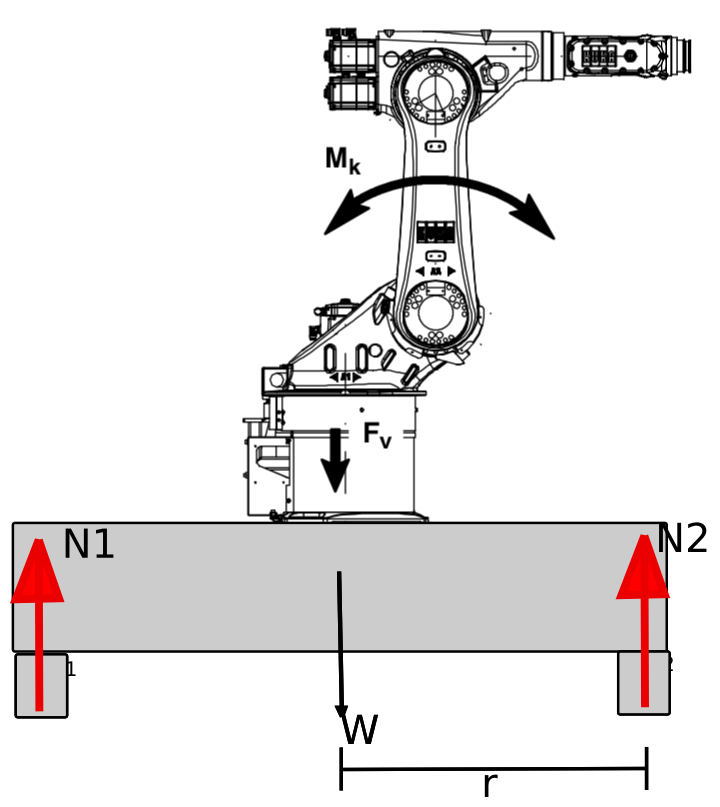
\includegraphics[width=0.5\columnwidth]{figs/base/tilt}
	\caption{Forças e torques máximos entre o robô e sua base.}
\end{figure}

Uma vez que a superfície do aro câmara e a região adjacente no tubo de sucção
são \textbf{ferromagnéticas}, é possível a utilização de bases magnéticas para
uma compensação do peso e raio necessário para a estabilização do robô. Os
dispositivos magnéticos se dispõem de duas maneiras para essa aplicação:
eletretromagnéticos e imãs permanentes. O primeiro caso tem como principal
vantagem a possibilidade de acionamento remoto, entretanto para situações de
falha em que haja perda de fornecimento de energia a força de atração também é
perdida. O segundo caso consiste em imãs permanentes arrumados de maneira que
seja possível organizar o fluxo magnético e, assim, controlar por meio de uma
alavanca a presença ou ausência de força magnética. A figura
\ref{figs/base/imas} ilustra os dois tipos de bases magnéticas citados.
Comercialmente, foram encontrados bases magnéticas com capacidade de até 3000N.

%TODO figura imãs













%\section{Compilação de questões}\label{sec:questoes}
Nesta seção, será apresentada a compilação das questões em aberto até o momento,
sendo de extrema necessidade a elucidação para a escolha da solução mais
apropriada e eficiente à aplicação. 


%\includepdf[pages=-]{articles/questoes.pdf}
\section{Estudo de viabilidade técnica}

O estudo de viabilidade consiste em avaliar as soluções conceituas mais simples 
da seção~\ref{sec:projeto}, ou seja, um estudo técnico específico para as
seguintes soluções: acesso pela escotilha superior com manipulador industrial de
pequeno porte e base customizada operada eletronicamente; acesso pela escotilha
inferior com manipulador industrial de médio porte e base fixa magnética; e
acesso pela jusante com manipulador industrial de grande porte e base fixa
magnética.

A primeira etapa do estudo de viabilidade consiste em pesquisa de mercado por
manipuladores industriais, levando em consideração os requisitos do processo de
metalização (velocidade e payload), espaço de trabalho, e as dimensões e peso
para compatibilidade com o acesso. O resultado da pesquisa mostrou que, em
relação ao acesso pela escotilha superior, as dimensões reduzidas restringiram muito a busca e apenas o
manipulador LBR 820 da Kuka satisfaz aos requisitos. Para os outros acessos, há
variadas soluções de manipuladores industriais.

As outras etapas são avaliações técnicas e são divididas nas seguintes
subseções: estudo geométrico para confirmar alcance do manipulador em todos os
pontos da pá; construção do ambiente 3D em SolidWorks, projeto de bases
mecânicas, movimentação e logística de acesso; simulação do espaço de trabalho e
e estudo de manipulabilidade; estudo de placas de sacrifício, mecanismos atuados
para interromper o revestimento e materiais. 

\subsection{Estudo geométrico}\label{sec::estudo_geom}
O estudo geométrico é uma avaliação simples de alcance dos manipuladores
industriais no ambiente do aro câmara. Tem como objetivo verificar se o
manipulador consegue percorrer todos os pontos da pá dentro das restrições da
tarefa HVOF, assumindo a pá planar, e diferentes posições de base. O estudo
leva em consideração as seguintes posições para o manipulador: escotilha
superior e base móvel; manipulador em frente à pá e base móvel verticalmente;
manipulador entre as pás e base móvel verticalmente.

Assumimos $R = 3.95 m$ e $R_m = 3 m$, onde $R$ é a distância do centro do cone à
superfície do aro câmara, e $R_m$ é o comprimento da pá. Logo, podemos
inferir o comprimento do aro câmara $P = 2*\pi *R = 24.81 m$. Em relação ao
centro do cone, o setor circular que cada pá ocupa tem um ângulo, em radianos,
de $\beta = \frac{R_m*2*\pi}{P} = 0.76$, e a metade do setor circular entre
as pás tem ângulo $\alpha = \pi/4$, já que elas são simetricamente distribuídas.
A figura~\ref{pa} mostra os parâmetros acima, onde as pás estão representadas
como setores circulares roxos e metade da distância entre as pás como setor
azul.

\begin{figure}[h!]
\centering
	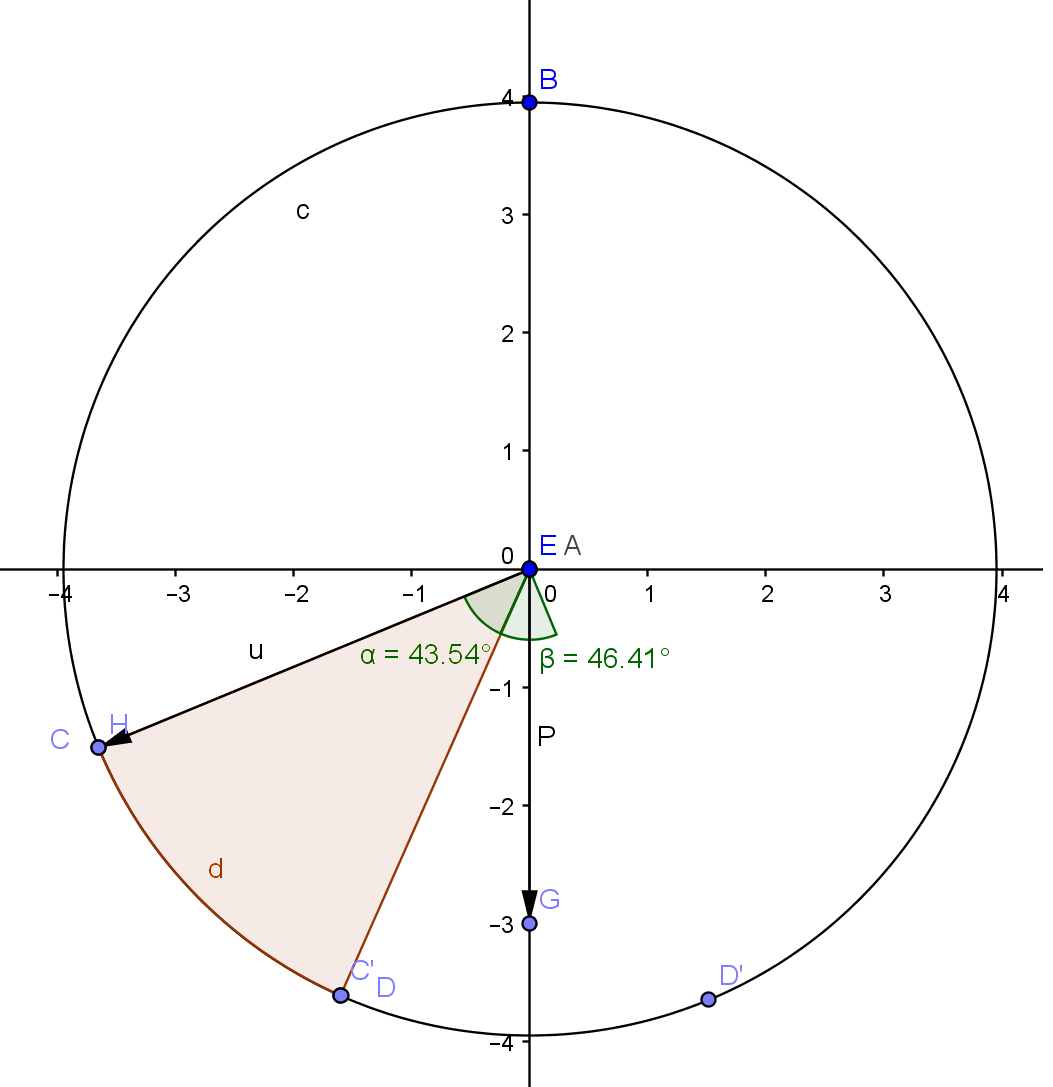
\includegraphics[width=\columnwidth]{figs/estudo/geometrico/pa.png} 
	\caption{Parâmetros do aro câmara.}
	\label{pa}
\end{figure}

Pode-se posicionar a base do manipulador em diferentes valores de $\alpha$, que é
o mesmo que girar a turbina e alterar a posição da pá. Para $\alpha = 0$, por
exemplo, o manipulador se encontra em frente à pá, e para $\alpha = \pi/4$ ele está entre as pás.

\subsubsection{Análise geométrica para a escotilha inferior}
A análise para a escotilha inferior consiste em posicionar o manipulador no
centro ou entre as pás ($\alpha = 0$ ou $\alpha = \pi/4$) e assumir $\omega =
\pi/4$ (pá girada $45^o$). No caso em que o
manipulador se encontra em frente à pá, alcançar todos os pontos da pá  é
traçar uma circunferência que a envolve, representando
a área de alcance do manipulador. Após o cálculo desta
circunferência, deve-se distanciar ortogonalmente a base do manipulador à pá,
pois este deve estar posicionado de uma maneira que não haja colisões. A
figura~\ref{paemfrente} mostra a circunferência, cujo raio pode ser encontrado
analiticamente pelas equações:
$$\rho ^2 = r^2+R_c^2-2R_crcos(\beta)$$
$$\rho ^2 = R^2+R_c^2-2R_cRcos(\beta)$$
onde $R$ é o raio do aro câmara, $r$ é o raio do cone da turbina, $R_c$ é a
distância do centro da pá ao centro do cone e $\rho$ é o raio da circunferência
que circunscreve a pá. Obtêm-se  $\rho=1.6387$ e $h=1.0157$, onde $h$ é a altura
da base do manipulador ($R-R_c$). Observe que $\rho$ é o alcance para o
manipulador sob a pá, logo temos que supor uma distância $d$ entre o manipulador
e a pá a fim de evitar colisões. Assumindo diversos valores para $d$, obtemos o
gráfico~\ref{reach} que mostra o alcance necessário do manipulador versus
distância que ele se encontra da pá. 

\begin{figure}[h!]
\centering
	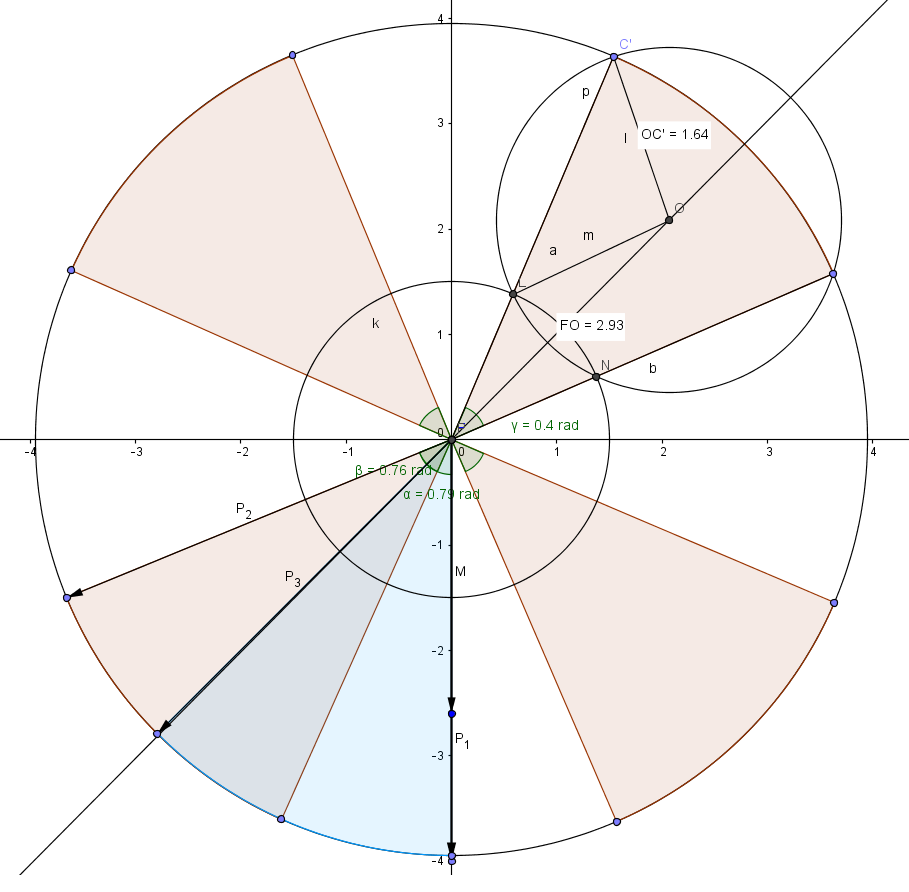
\includegraphics[width=\columnwidth]{figs/estudo/geometrico/paemfrente.png} 
	\caption{Estudo geométrico do manipulador industrial em frente à pá.}
	\label{paemfrente}
\end{figure}

\begin{figure}[h!]
\centering
	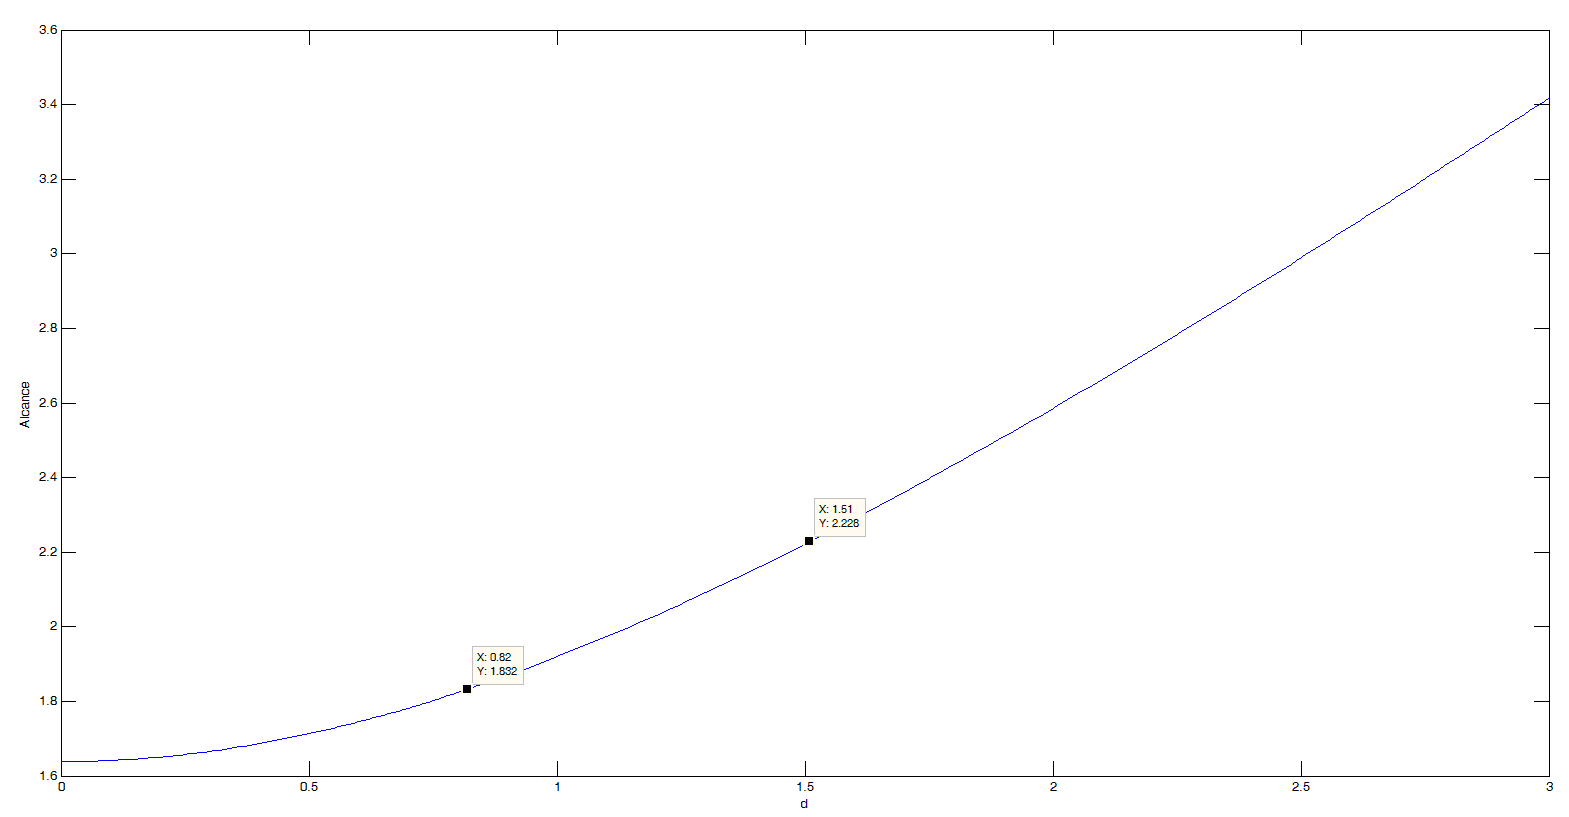
\includegraphics[width=\columnwidth]{figs/estudo/geometrico/reach.png} 
	\caption{Gráfico que mostra o alcance necessário do manipulador versus a
	distância que ele se encontra da pá.}
	\label{reach} 
\end{figure}

Para uma posição fixa da base, o manipulador, a uma distância de 1 m
da pá, necessita ter alcance máximo de 1.7 m para percorrer todos os pontos, se
considerarmos os 230 mm de distância mínimo entre pá e pistola. Esta é uma
solução inviável para um manipulador de médio porte e com o payload necessário.
Portanto, será realizada uma análise mais profunda levando em consideração
possibilidade de movimentação da base horizontalmente por atuador ou
manualmente.

\subsubsection{Análise geométrica para a escotilha superior}
Na escotilha superior, como há restrição em relação ao manipulador (LBR 820), há
a necessidade de uma base móvel, que possa assumir diversos comprimentos e
posições. A solução de uma base com dois elos está representada na
figura~\ref{pakuka}, onde os elos i e j estão representados em verde, o cone
da turbina representado pela circunferência c, o espaço de trabalho planar do
manipulador está representado em verde, e a pá representada como um setor
circular em vermelho.

\begin{figure}[h!]
\centering
	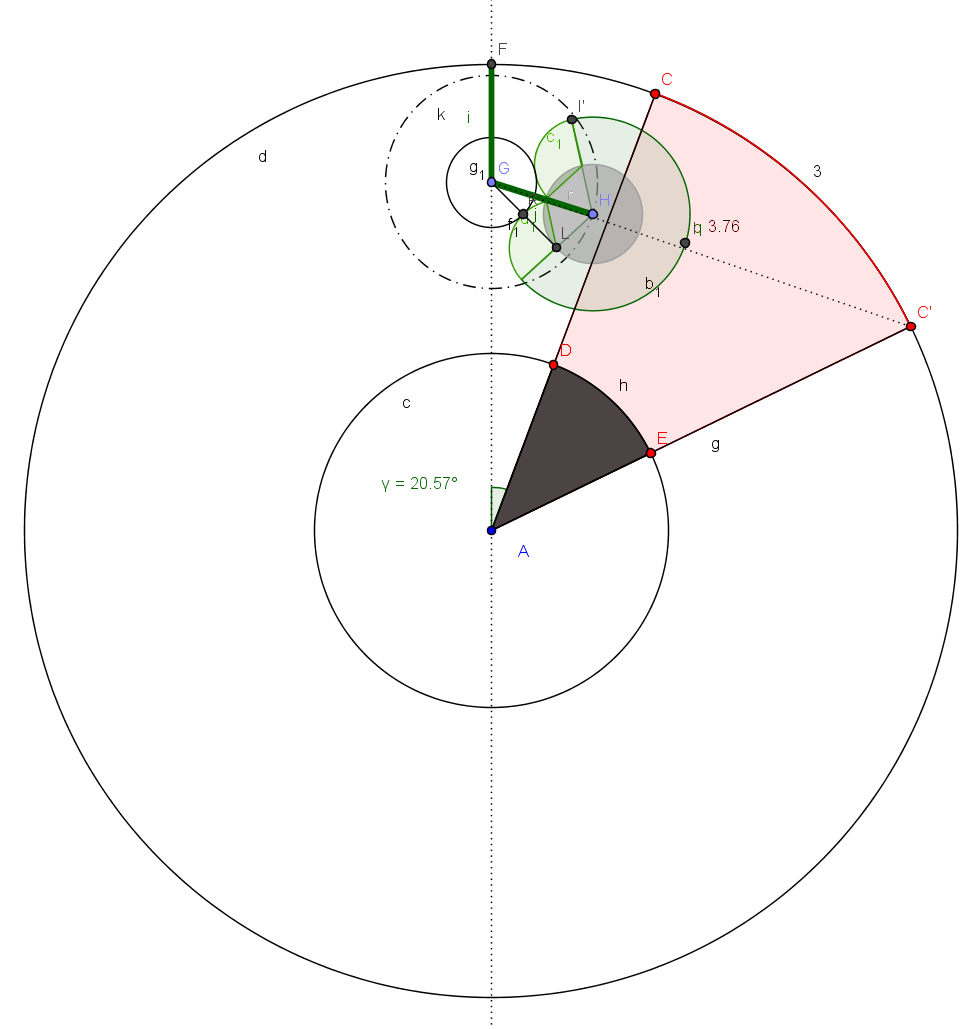
\includegraphics[width=\columnwidth]{figs/estudo/geometrico/kuka.png} 
	\caption{Estudo geométrico do manipulador industrial Kuka 820 na escotilha
	superior e base de dois elos.}
	\label{pakuka}
\end{figure}

Utilizando notação vetorial, considere: 
$$\overrightarrow{Z}=(0,0,1)$$
$$\overrightarrow{X}=(1,0,0) $$
$$\overrightarrow{Y}=(0,1,0)$$
$$\overrightarrow{P_0} = (0,R,0)$$
$$\overrightarrow{P_c}=(0,R-x,0)$$
$$\overrightarrow{\widetilde{P}} = R_z(-\alpha) \overrightarrow{P_0}$$
$$\overrightarrow{\overline{\widetilde{P}}}=\frac{\overrightarrow{\widetilde{P}}}{\left \| \overrightarrow{\widetilde{P}} \right \|}$$
$$\overrightarrow{P_R} =R_{\overrightarrow{\overline{\widetilde{P}}}}(\omega)R_z(-(\alpha+\beta/2)P_0$$
$$\overrightarrow{v}=R_{\overrightarrow{\overline{\widetilde{P}}}}(\omega)R_z(\beta/2)R_z(-\alpha)\overrightarrow{Y}$$
$$\overrightarrow{P_a} =R_{\overrightarrow{\overline{\widetilde{P}}}}(\omega)\overrightarrow{Z}$$
$$P_{r} = P_R\frac{r}{R}+\overrightarrow{P_a}*0.23$$
$$P_R =P_R+0.23 $$

onde $\overrightarrow{P_0}$ é o vetor do centro do cone ao acesso superior,
$\overrightarrow{P_c}$ é o vetor do centro do cone ao fim do primeiro elo da
base i, $\overrightarrow{\widetilde{P}}$ é o vetor do centro do cone da turbina
ao aro câmara que passa pelo centro da pá,
$\overrightarrow{\overline{\widetilde{P}}}$ é o vetor unitário correspondente a
$\overrightarrow{\widetilde{P}}$, $\overrightarrow{P_R}$ é o vetor do centro do cone da turbina
ao extremo superior da pá, $\overrightarrow{v}$ é um vetor unitário no plano da
pá e no extremo superior, $\overrightarrow{P_r}$ é o vetor do centro do cone da
turbina ao extremo inferior da pá ,$\overrightarrow{P_a}$ é um vetor unitário
normal à pá, $R_z$ é rotação em torno de $\overrightarrow{Z}$, $\omega$ é o
ângulo de rotação da pá em seu próprio eixo (valor que pode variar de $0$ a
$45^o$), $x$ é o comprimento do elo i e $y$ é o comprimento do elo j.

O projeto consiste em encontrar o valor de $y$ (comprimento do segundo elo da
base) para diferentes valores de $x$ (elo i). O elo possui uma junta
prismática, portanto, $y$ assume valores mínimos para alcançar o extremo
inferior da pá, e máximos para alcançar o extremo superior da pá.
Utilizando as dimensões do Kuka LBR, resolve-se a equação: 
$$y = max (\left \|
\overrightarrow{P_R}-\overrightarrow{P_c} \right \|, \left \|
\overrightarrow{P_r}-\overrightarrow{P_c} \right \|) - 1.18$$ 
Com ajuda computacional e percorrendo todos os valores de  $\alpha$ e $x$,
obtém-se o gráfico~\ref{yminsmallhatch}. Em vermelho, temos o comprimento máximo do elo e,
em azul, o comprimento mínimo, recolhido, do elo com junta prismática. Observe
que para valores de $\alpha$ menores que 13.86 graus não há solução viável e,
para valores entre 14 e 40 graus o elo estendido é maior que o dobro do elo
reduzido, o que dificulta a solução também.

\begin{figure}[h!]
\centering
	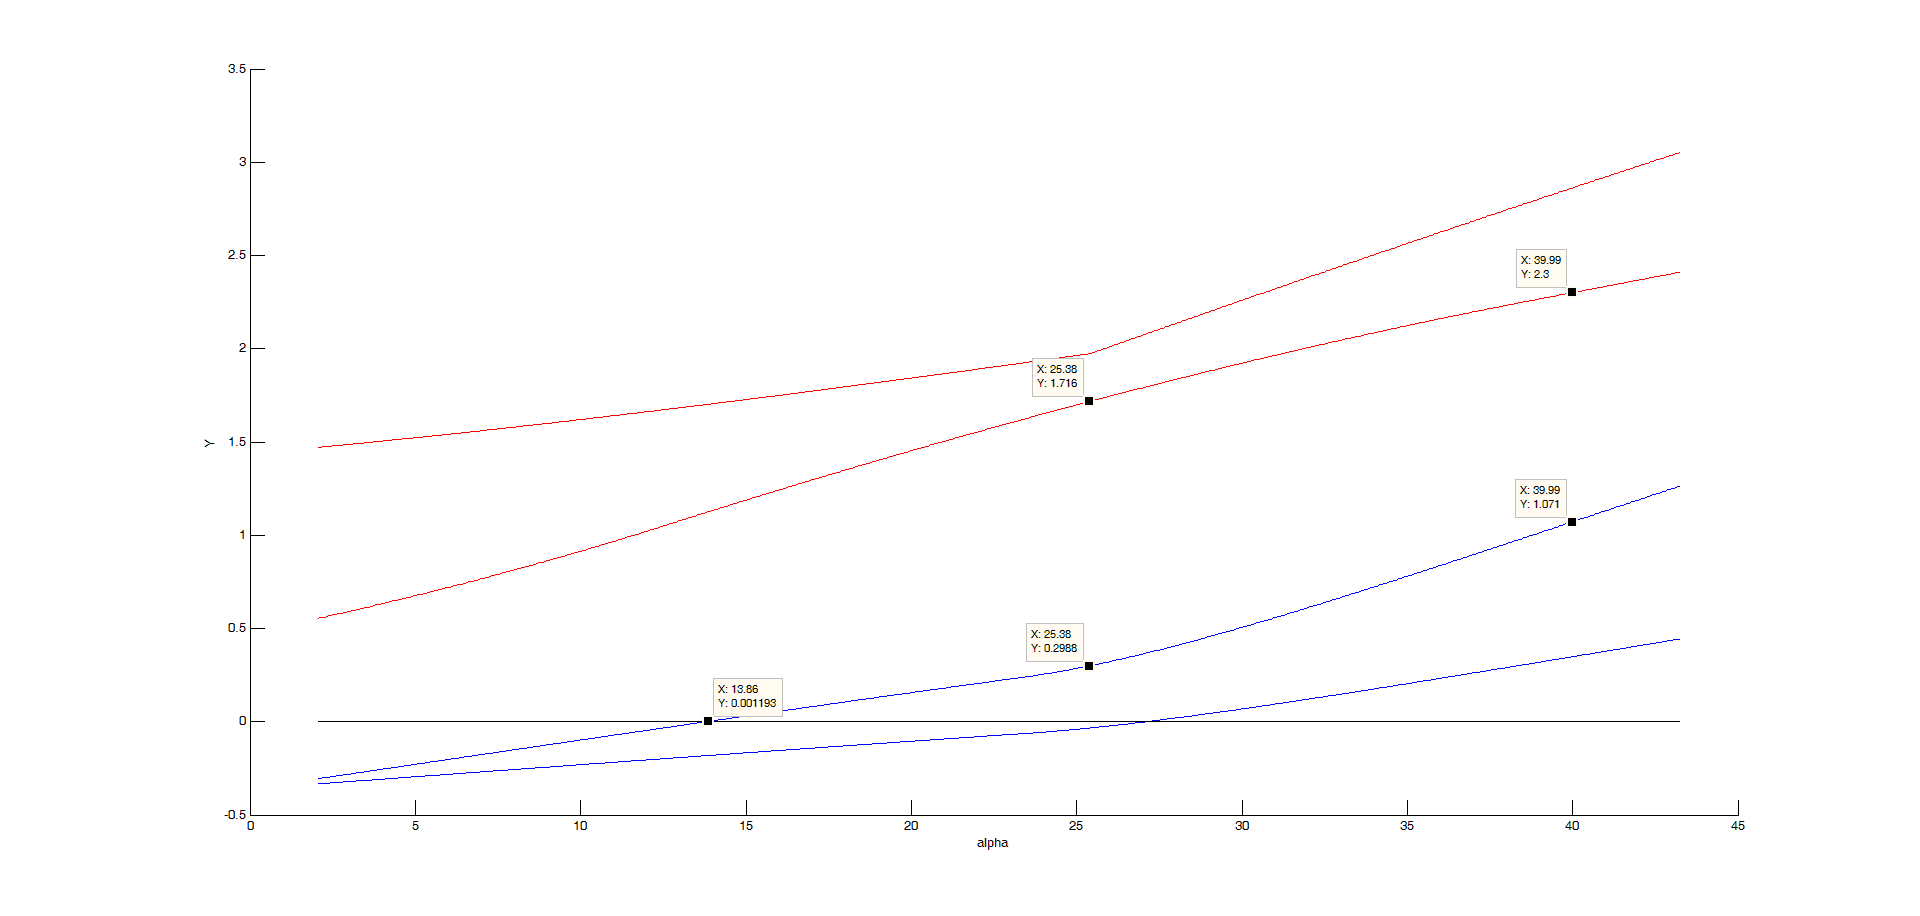
\includegraphics[width=\columnwidth]{figs/estudo/geometrico/yminsmallhatch.png} 
	\caption{Estudo do comprimento mínimo e máximo para o segundo elo da base.}
	\label{yminsmallhatch}
\end{figure}

A análise puramente geométrica não considera o formato real curvilíneo da pá e
é apenas uma análise de alcance de extremos. Isso não garante que a área de
trabalho do manipulador cubra todos os pontos da pá e ainda não considera
algumas colisões com o ambiente e/ou própria base e manipulador. O estudo do
espaço de trabalho por simulações se faz necessário para garantir a viabilidade
dos manipuladores industriais.
\subsection{Modelagem 3D das soluções}
Os estudos das possíveis soluções exigiu uma visualização mais detalhada do
volume livre no interior da turbina. Para isso, foi recriado o ambiente da
turbina em CAD 3D no SolidWorks, a partir dos desenhos 2D de seção da turbina
fornecidos pelo cliente.
O modelo tridimensional do aro câmara permite o estudo e o dimensionamento geométrico de
alcance do manipulador para cada solução. Não foram necessários
detalhamentos de todos os componentes, podendo ser apenas considerados, e
representados com maior precisão, os perfis externos do túnel à montante, o
estator, o rotor e uma pequena região à jusante, além dos acessos
por escotilha superior e inferior.
A figura~\ref{fig::ambiente3d} apresenta o ambiente da turbina em CAD e os
possíveis acessos para realização das intervenções.

\begin{figure}[h!]
\centering
	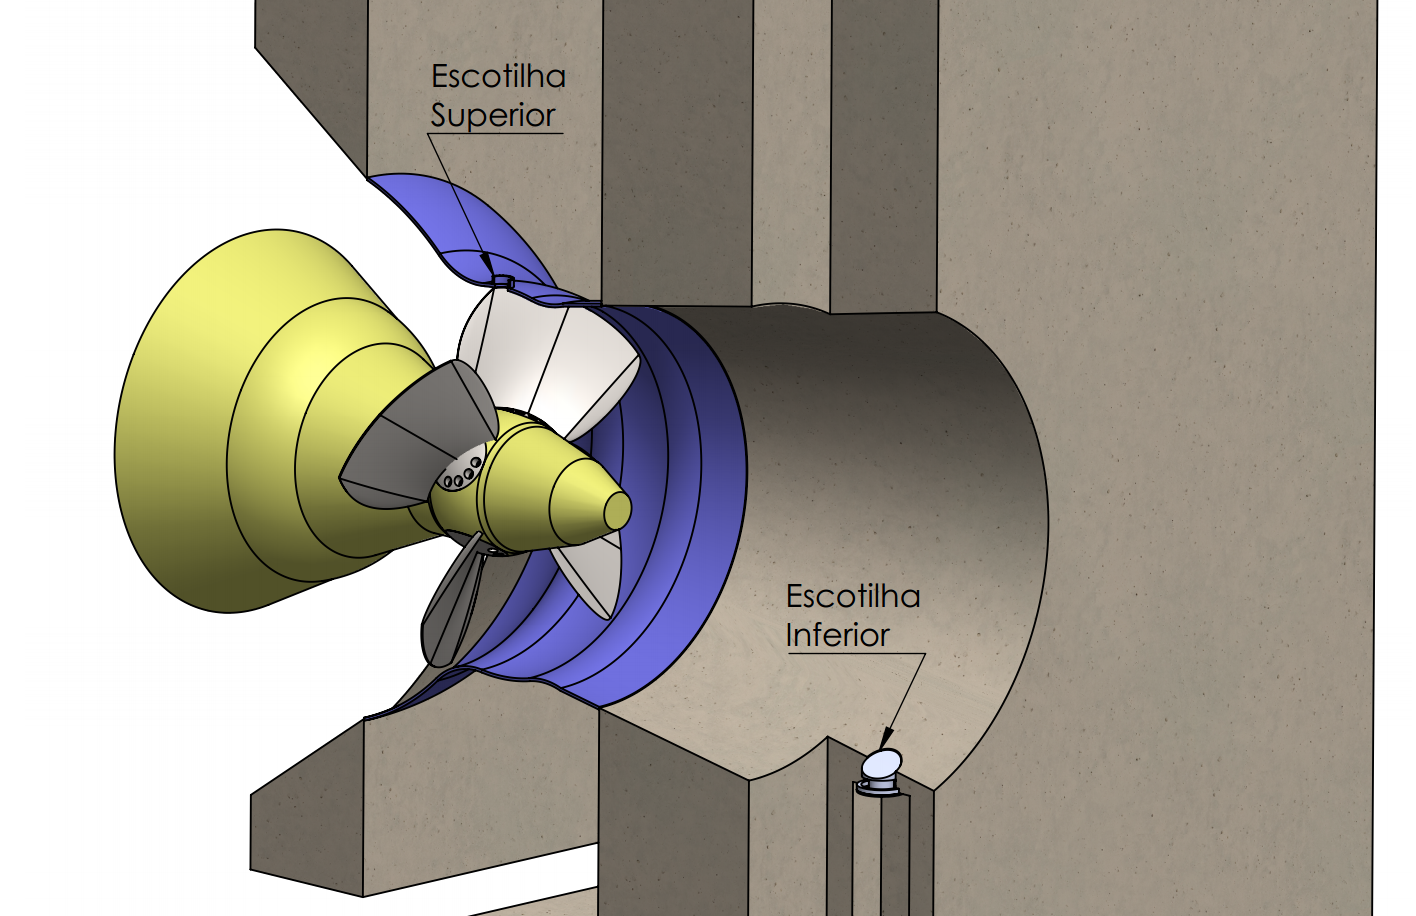
\includegraphics[width=\columnwidth]{figs/estudo/solid/ambiente_3d} 
	\caption{Ambiente 3D da Turbina, em SolidWorks}
	\label{fig::ambiente3d}
\end{figure}

A solução pela escotilha superior, devido ao espaço reduzido de entrada, não
permite a utilização de manipuladores de grande porte, sendo escolhido o KUKA
LBR 820. Este manipulador não possui alcance para realizar a operação em toda a
pá de uma só vez, exigindo uma base customizada que permita o
posicionamento do manipulador para realização das operações por etapas. Para
isso, foi estudada uma estrutura de base que permitisse diferentes
posicionamentos para o manipulador no interior do aro câmara, de forma que este
pudesse cobrir toda a superfície da pá. A base consiste em 3 braços
telescópicos que permitem a extensão do sistema para prover o alcance
necessário ao manipulador e o recolhimento para uma configuração incial que
permita a entrada do manipulador no aro câmara com segurança, sem o risco de
choques ou interferências indesejadas. Além disso, uma junta rotativa oferece mais um grau
de liberdade para o sistema, facilitando o acesso do manipulador à toda ar
superfície da pá. Os atuadores são acionados eletricamente com sensor de
posicionamento. Atuadores de esferas recirculantes foram escolhidos devido à
baixa folga e precisão elevada. A estrutura da base é composta por cilindros de
diâmetro maximizado e pequena espessura, o que oferece um momento de inércia
polar elevado e baixo peso, fornecendo grande rigidez à flexão e minimizando
assim erros de posicionamento e vibração excessiva. A
figura~\ref{fig::base_recolhida} e a figura~\ref{fig::base_extendida} apresentam
o conceito da base do manipulador em duas configurações: recolhida (configuração
de entrada) e extendida (configuração de operação).

\begin{figure}[h!]
\centering
	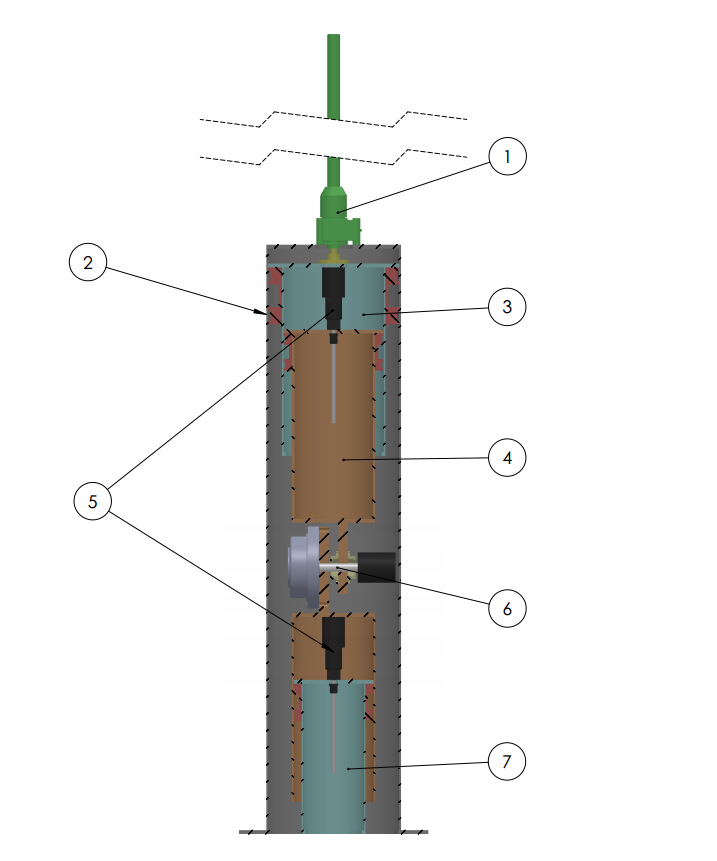
\includegraphics[width=\columnwidth]{figs/estudo/solid/Base_Recolhida.PNG} 
	\caption{Detalhes em corte da base na configuração inicial recolhida}
	\label{fig::base_recolhida}
\end{figure}

\begin{figure}[h!]
\centering
	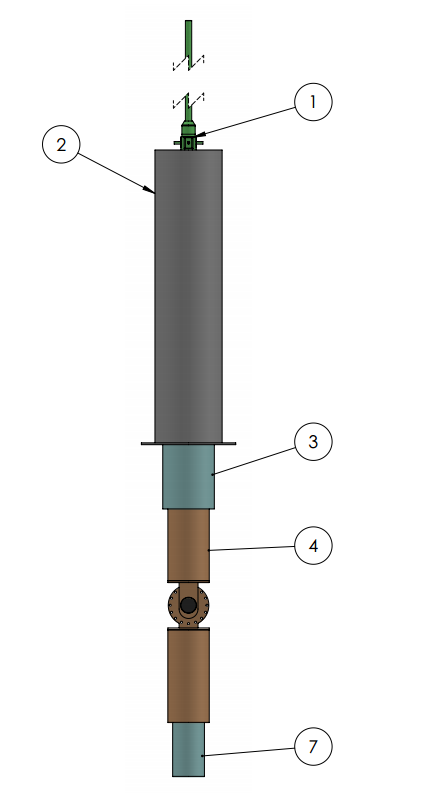
\includegraphics[width=\columnwidth]{figs/estudo/solid/Base_Extendida.PNG} 
	\caption{Base na configuração totalmente extendida}
	\label{fig::base_extendida}
\end{figure}

Os componentes principais da base estão representados nas
figuras~\ref{fig::base_recolhida} e~\ref{fig::base_extendida}, são: 1.atuador
linear por sem-fim coroa; 2.base fixa; 3.braço prismático \#1; 4.braço
prismático \#2; 5.atuadores lineares; 6.junta rotativa; 7.braço prismático \#3.

A figura~\ref{fig::base_ambiente3d_recolhida} demonstra a base com o
manipulador KUKA LBR 820 e as dimensões extremas, em milímetros, estimadas para o
interior e para fora da turbina, na configuração inicial de entrada no aro
câmara pela escotilha superior.
A figura~\ref{fig::base_ambiente3d_extendida} apresenta a base com o manipulador
em uma configuração qualquer de operação, demonstrando o ganho de alcance e
generalidade de posicionamento fornecidos pela base.

\begin{figure}[h!]
\centering
	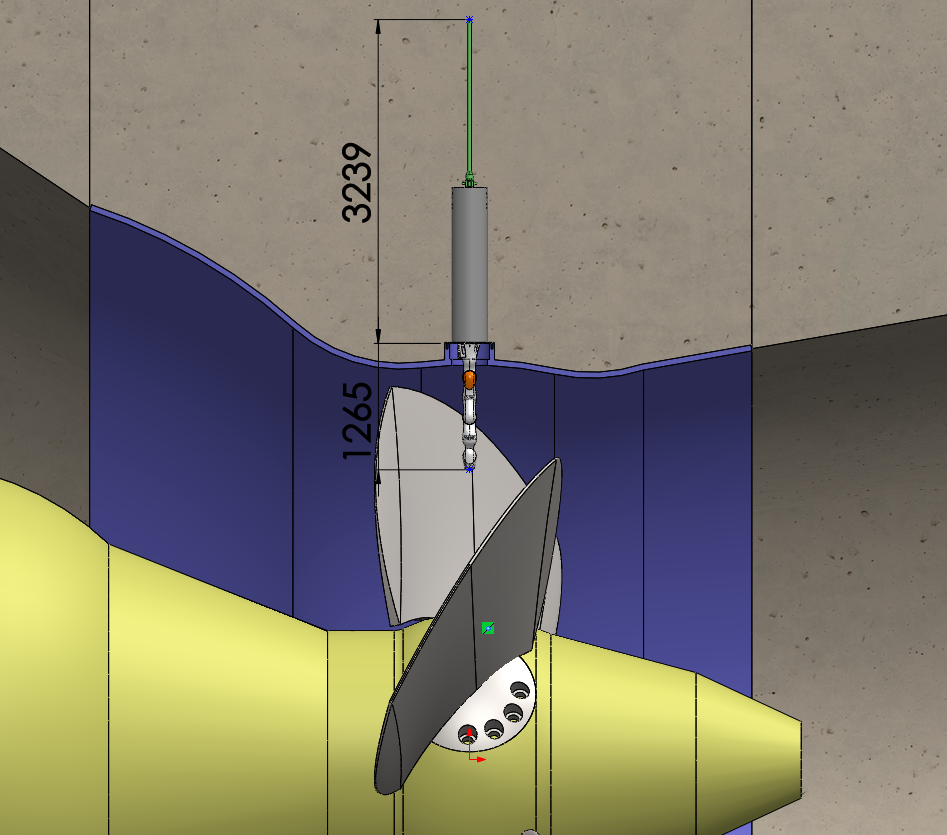
\includegraphics[width=\columnwidth]{figs/estudo/solid/Base_Ambiente3d_Recolhida.png} 
	\caption{Base na configuração inicial no ambiente da turbina}
	\label{fig::base_ambiente3d_recolhida}
\end{figure}

\begin{figure}[h!]
\centering
	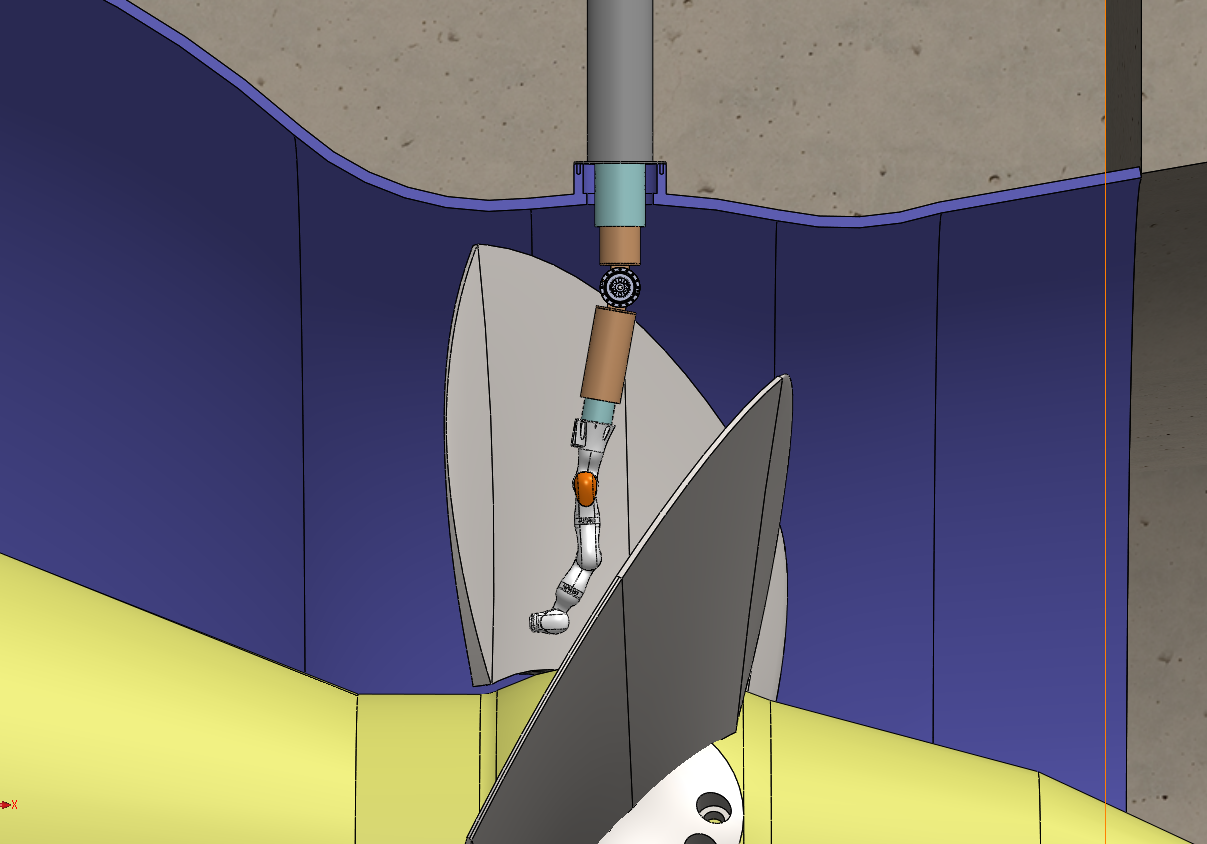
\includegraphics[width=\columnwidth]{figs/estudo/solid/Base_Ambiente3d_Operacao.PNG} 
	\caption{Base em uma geral configuração de operação}
	\label{fig::base_ambiente3d_extendida}
\end{figure}








 
\subsection{Estudo do espaço de trabalho do manipulador}

Para uma avaliação técnica das soluções é necessária a análise do espaço de
trabalho, assim como a manutenção de sua manipulabilidade em toda a trajetória a
ser traçada. A escolha de um manipulador industrial, no contexto da aplicação
desejada, é um compromisso entre o tamanho do manipulador e o espaço disponível.
Um manipulador de grande porte garante que todos os pontos a serem metalizados
sejam processados sem problemas, entretanto pode tornar inviável que o mesmo se
movimente no espaço confinado e consiga passar pelos acessos limitados. Por esse
motivo, é necessário que a escolha do manipulador seja ótima no aspecto do
tamanho do manipulador e de seus graus de liberdade, para que seja possível de
se especificar o menor manipulador possível que atenda com uma certa margem de
segurança a tarefa a ser realizada.

A análise do espaço de trabalho do manipulador será realizada utilizando-se
ferramentas de simulação 3D específicas para manipuladores robóticos. No
processo de estudo de viabilidade técnica serão utilizados dois
\textit{frameworks:} \textit{OpenRAVE - Open Robotics Automation Virtual
Environment}, utilizado para uma análise detalhada do espaço de trabalho do
robô e o \textit{MoveIt!}, utilizado principalmente para o planejamento e
análise de trajetórias e controle de manipuladores.

A primeira etapa no estudo consiste na importação dos modelos desenvolvidos em
\textit{SolidWorks} para o ambiente de simulação do \textit{OpenRAVE}. O Aro
câmara e o rotor tem papel fundamental na descrição do espaço disponível para a
realização do processo de metalização. A figura \ref{fig::rotor_openrave}
ilustra o aro câmara e o rotor no ambiente de simulação do \textit{OpenRAVE}. 

\begin{figure}[h!]
\centering
	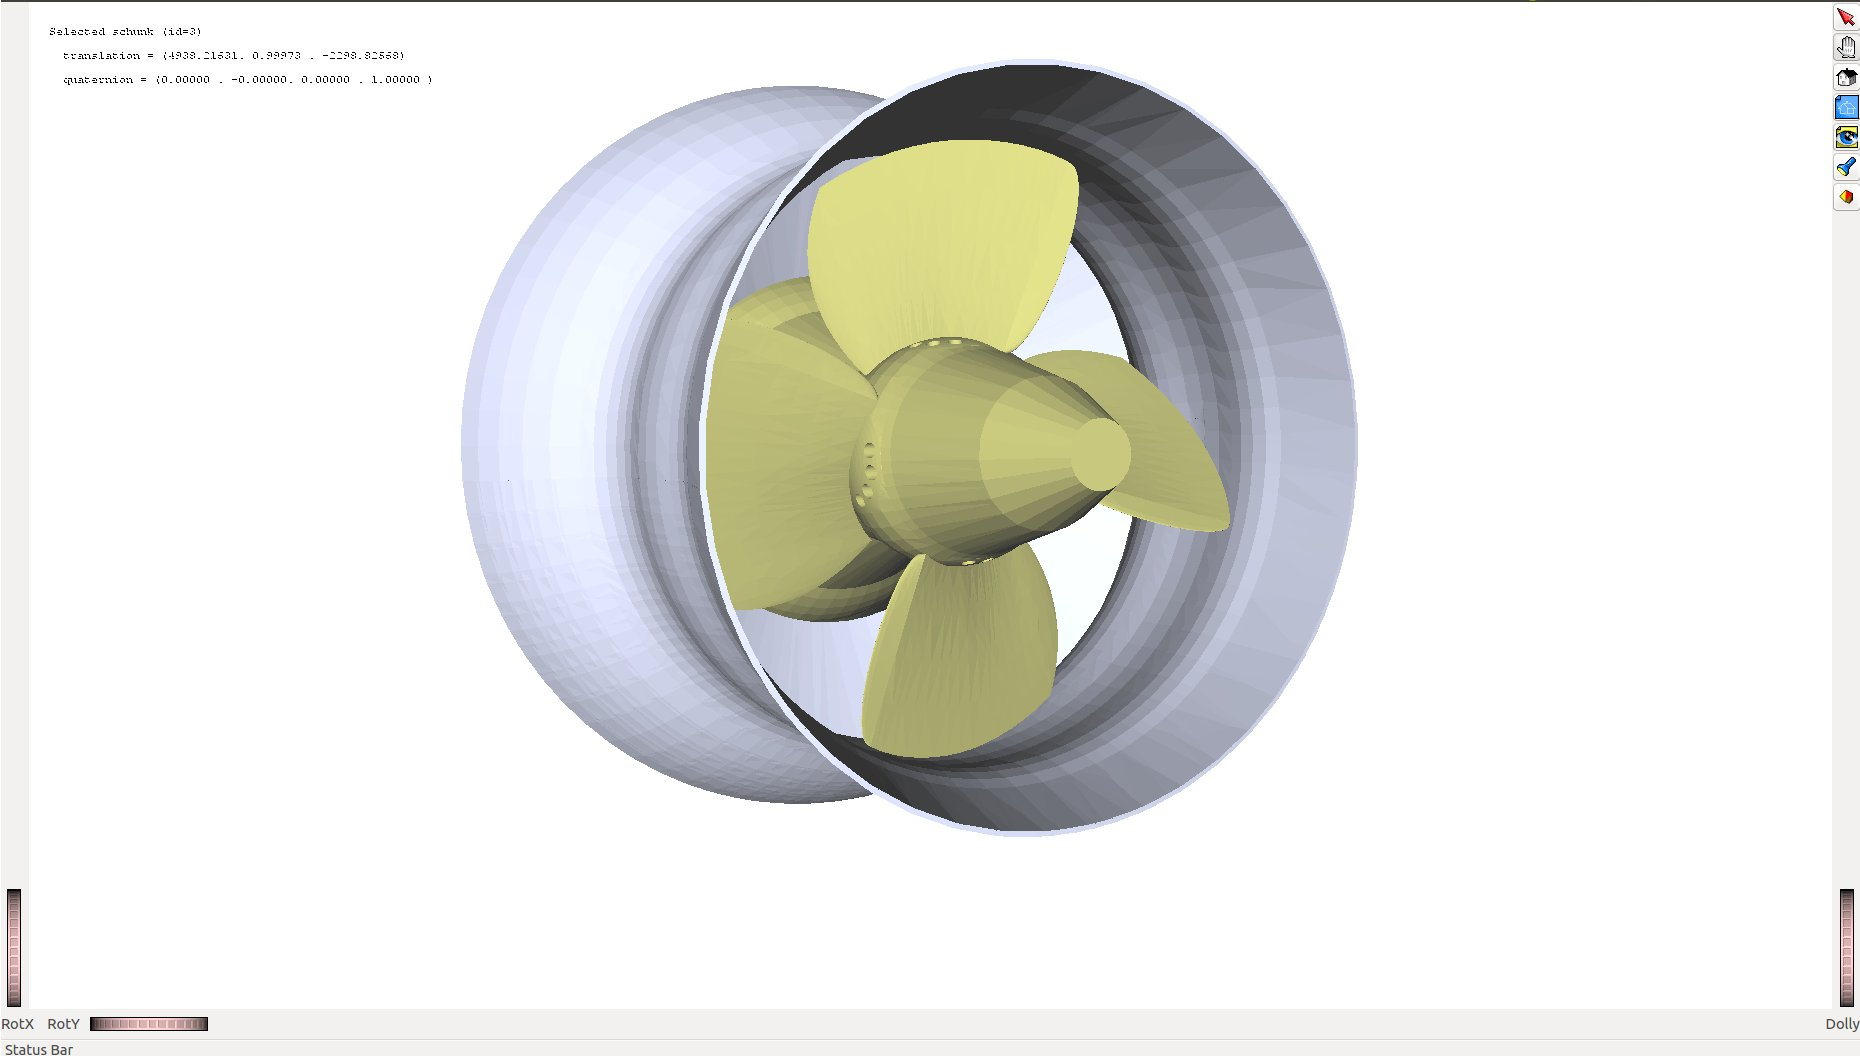
\includegraphics[width=\columnwidth]{figs/openrave/rotor_openrave}
	\caption{Turbina simulada no ambiente do \textit{OpenRAVE}.}
	\label{fig::rotor_openrave}
\end{figure}

Cada manipulador robótico a ser simulado deve ter sua estrutura modelada e suas
juntas assinaladas. Cada elo do robô deve ser modelado ou importado de um
arquivo externo e sua posição referente ao eixo de coordendas da base do
manipulador, assim como o eixo de rotação e os ângulos
limites de cada junta devem ser descrito de maneira a formar uma representação
completa do manipulador no ambiente de simulação. Para uma primeira análise,
foram escolhidos dois manipuladores industriais padrão com dimensões dentro de
faixas que representassem um manipulador de médio e grande porte. Como
manipulador de médio porte foi escolhido o modelo \textit{KR 30} do fabricante
\textit{Kuka Robotics} e para o manipulador de grande porte o modelo
\textit{KR 30l16}, do mesmo fabricante, foi selecionado.
A escolha desses manipuladores é justificada, em um primeiro momento, para uma
familiarização com o ambiente de simulação e uma perspectiva das dimensões
necessárias e limites para manipuladores industriais. 

O manipulador \textit{Kr30} é um manipulador de médio porte, com capacidade de
30kg de carga, 45kg de carga adicional, alcance máximo de 2033mm. A figura
\ref{fig::kukakr30_openrave} ilustra o modelo gerado no ambiente de simulação. 

\begin{figure}[h!]
\centering
	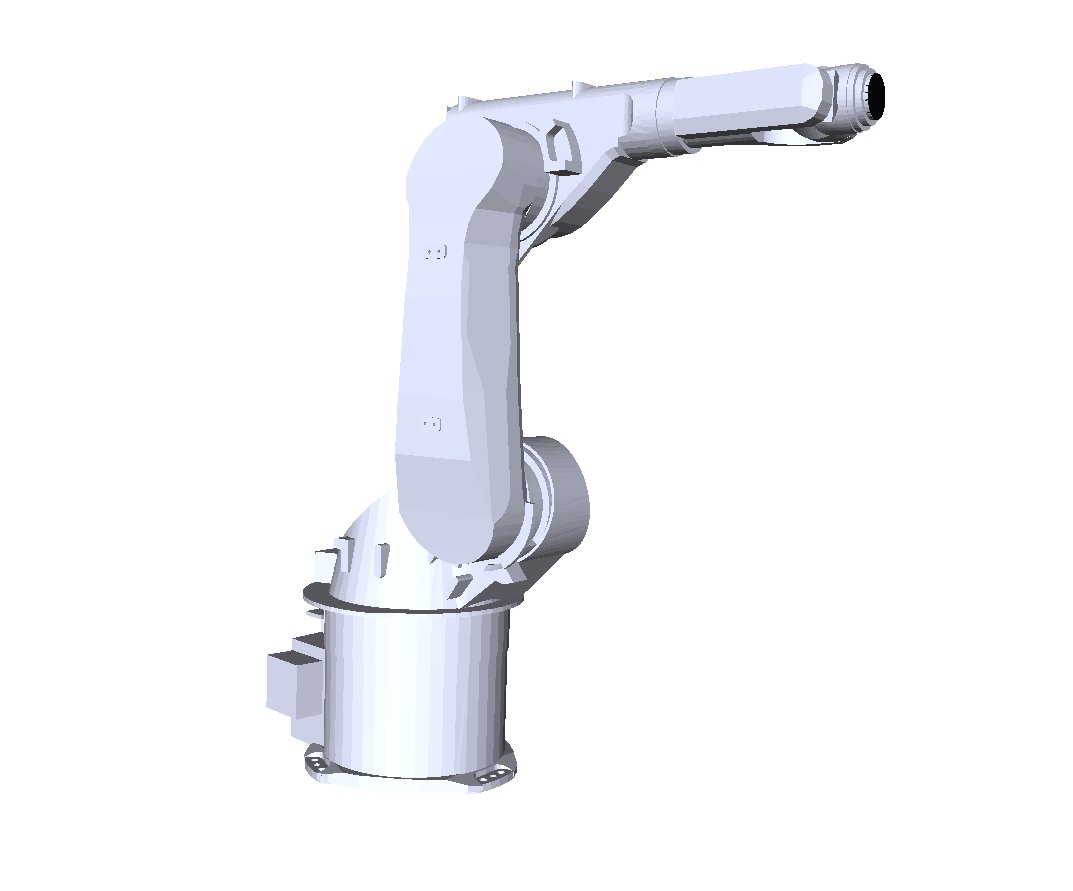
\includegraphics[width=0.8\columnwidth]{figs/openrave/kukakr30_openrave}
	\caption{Manipulador industrial modelo Kuka-KR30 no ambiente de simulação.}
	\label{fig::kukakr30_openrave}
\end{figure}

Por sua vez, o manipulador de grande porte, ilustrado na figura
\ref{fig::kukakr30l16_openrave} é uma versão extendida do manipulador \textit{KR
30} com alcande de 3102mm e carga reduzida para 16kg no efetuador e 45kg de carga adicional. Mesmo com a redução de carga o manipulador ainda se
encontra dentro de uma região aceitável, visto que o peso do sistema de
metalização é de 8,5kg.

\begin{figure}[h!]
\centering
	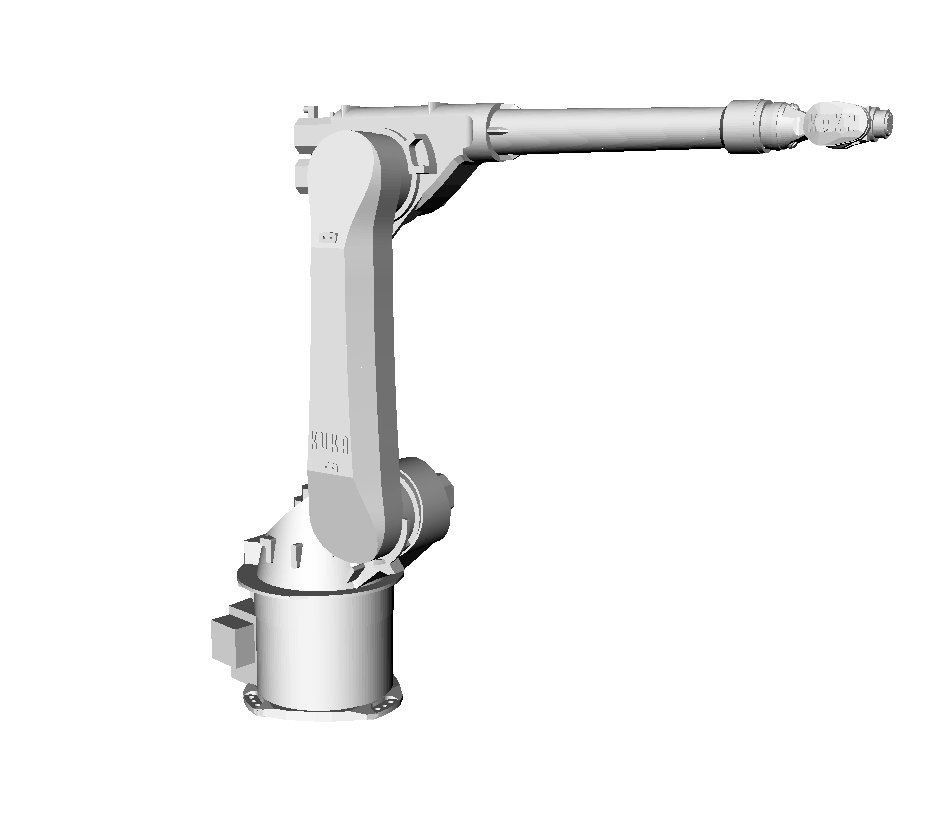
\includegraphics[width=0.8\columnwidth]{figs/openrave/kukakr30l16_openrave}
	\caption{Manipulador industrial modelo Kuka-KR30l16 no ambiente de simulação.}
	\label{fig::kukakr30l16_openrave}
\end{figure}

A especificação do alcance máximo do robô provê apenas a informação do ponto
mais distante de sua base que o manipulador consegue alcançar. Para a descrição
geométrica do espaço de trabalho, é necessário observar cada junta de revolução
ou prismática do robô e, também o tamanho dos elos. A partir dessas informações
é possível gerar um envelope que englobe todo o espaço em que é possível que o
manipulador se posicione. Entretanto, para o contexto da metalização, no qual a
tarefa a ser realizada impõe restrições de posição, orientação e velocidade, é
necessário analisar também a manipulabilidade do manipulador em cada posição.
Utilizando-se o ambiente de simulção do \textit{OpenRAVE} é possível gerar,
numericamente, uma representação visual em 3 dimensões do espaço de trabalho e
também do graus de liberdade em cada ponto do epaço. Esse estudo possibilita,
rapidamente, um entendimento básico do comportamento do robô dentro de seu
espaço de trabalho e também proporciona uma maior capacidade de discernimento do
posicionamento da base do robô para que a seja possível um melhor aproveitamento
do manipulador. A figura \ref{fig::workspace_openrave} ilustra o espaço de
trabalho do manipulador \textit{Kuka KR 30l16}, na qual o robô se
encontra no centro da esfera e cada ponto em que o manipulador consegue
alcançar é representado por uma cor, sendo que quanto mais vermelhor mais graus
de liberdade o efetuador possuí naquela posição.

\begin{figure}[h!]
\centering
	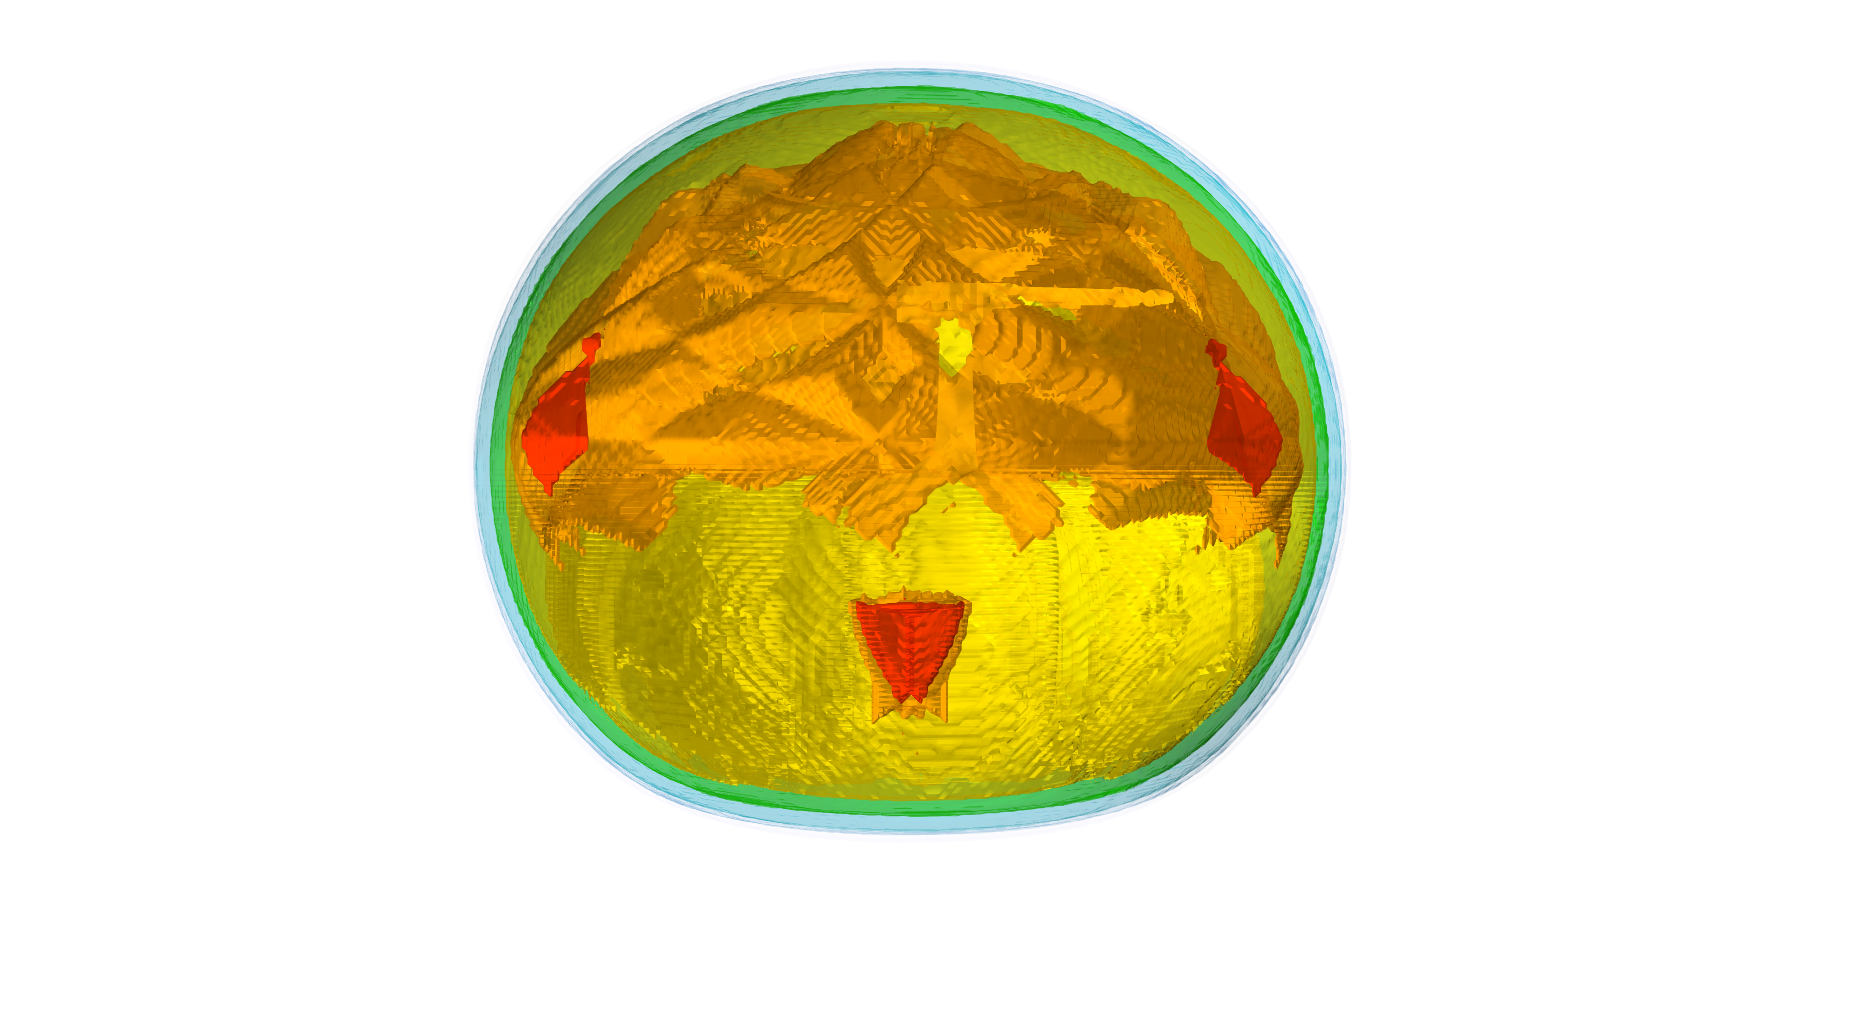
\includegraphics[width=\columnwidth]{figs/openrave/workspace_kr30l16_openrave}
	\caption{Representação do espaço de trabalho do Manipulador industrial
	modelo Kuka-KR30l16.}
	\label{fig::workspace_openrave}
\end{figure}

Uma vez que o ambiente de simulação foi configurado, é possível testar diversos
cenários com os diferentes manipuladores já modelados. Essa característica
proporciona uma análise superficial e validação de conceitos e, também, o teste
de posicionamento de manipuladores com detecção de colisôes. A figura
\ref{fig::position_test_openrave} ilustra a validação de posicionamento do
manipulador \textit{Kuka KR 30} para um ponto extremo da pá. 

\begin{figure}[h!]
\centering
	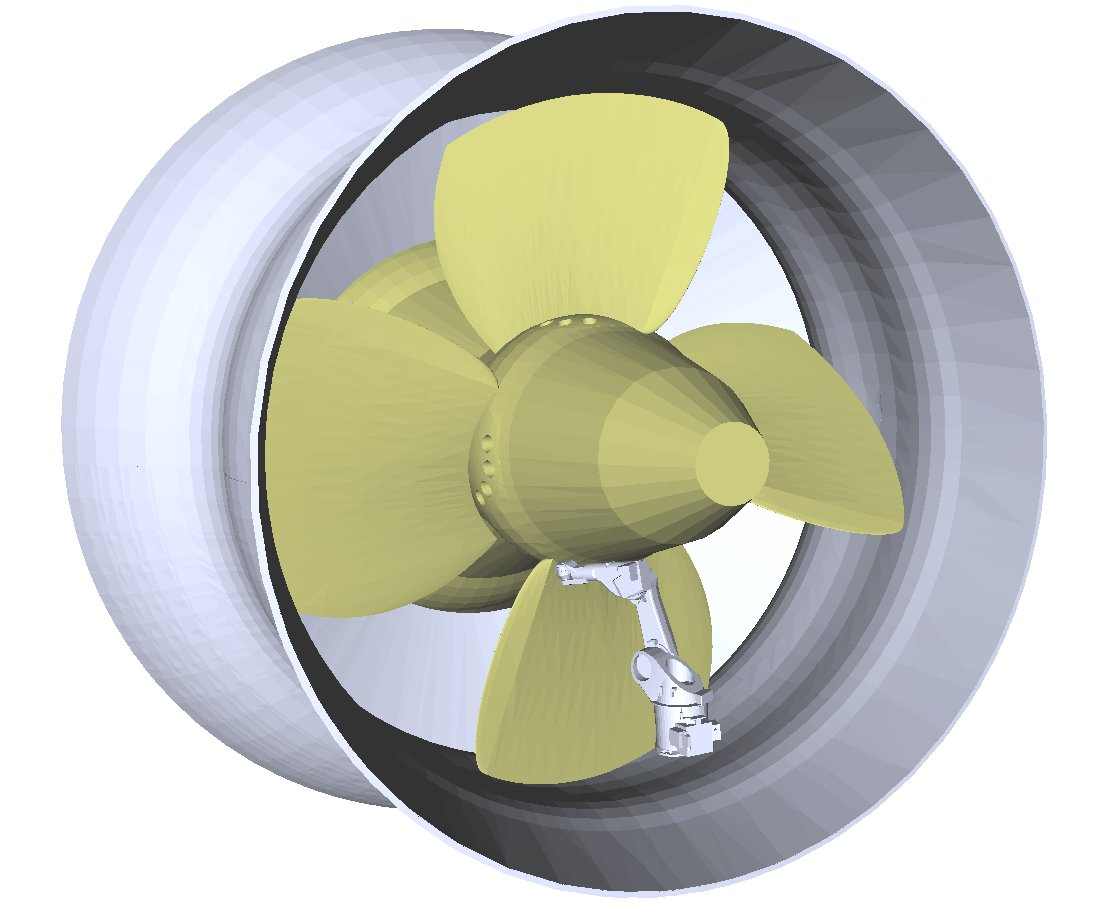
\includegraphics[width=\columnwidth]{figs/openrave/position_test_openrave}
	\caption{Representação do espaço de trabalho do Manipulador industrial
	modelo Kuka-KR30l16.}
	\label{fig::workspace_openrave}
\end{figure}

Após uma primeira análise verificou-se uma dificuldade de posicionamento do
modelo \textit{Kuka KR 30} de maneira que fosse possível a metalização completa
de uma face da pá do rotor sem a necessidade de movimentação da base. Por outro
lado, a utilização de uma manipulador de grande porte, como o \textit{Kuka KR
30l16}, torna-se muito complexa para o processamento das faces voltadas para a
Jusante, pois o espaço confinado entre as pás dificulta a movimentação do
manipulador. \textbf{O referencial zero para o ângulo das pás não foi
fornecido e foi utilizado o ângulo de $45^o$ em relação a linha perpendicular ao
fluxo d'água como posição de maior arbertura}. Com as informações geradas até o
momento, não é possível descartar a viabilidade técnica de nenhuma das soluções
e um estudo mais detalhado do posicionamento ótimo .a base do manipulador deverá
ser realizado, afim de se obter o menor número de movimentações para um
manipulador de médio porte e, também, a verificação de uma posição viável para o
processamento completo da parte à Jusante da pá utilizando-se um manipulador de
grande porte.

\subsubsection{Dimensionamento da base}

Para manipuladores com longo alcance, as forças e torques envolvidos requerem
uma estrutura de fixação do robô de forma que o sistema como um todo não se
movimente e, no caso extremo, tombe. Normalmente, os manipuladores robóticos são
fixados no chão e as características da superfície e tamanho dos parafusos
necessários são estipulados pelo fornecedor a partir dos valores máximos de
torque e força que o manipulador pode exercer em seu ponto de apoio.
Considerando um manipulador centrado em uma base circular apoiada no chão, dois
fatores influenciam capacidade de estabilização da estrutura: o raio da base e o seu peso.

O raio da base $r_{b}$ é limitado pelo ambiente da turbina e para cada escolha
de posicionamento existem restrições específicas. 
Para a realização dos cálculos de dimensionamento foi considerado,
primeiramente, o manipulador posicionado em frente a pá, como ilustrado na
figura \ref{fig::robot_front}.

\begin{figure}[h!]
\centering
	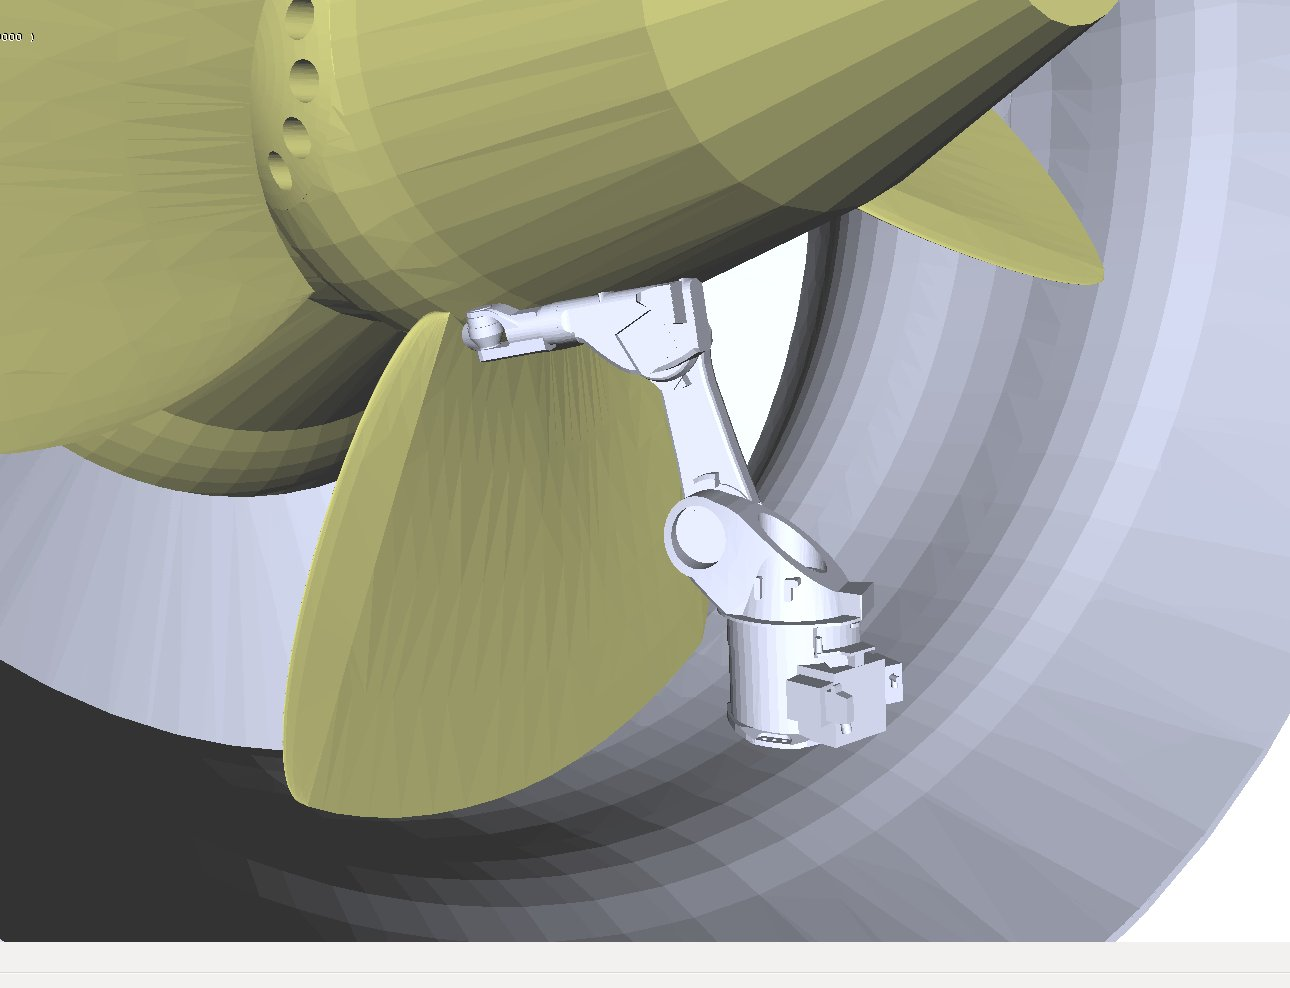
\includegraphics[width=0.9\columnwidth]{figs/openrave/robot_front_openrave.jpg}
	\caption{Exemplo de posicionamento de um manipulador robótico em frente à pá.}
	\label{fig::robot_front}
\end{figure}

 %TODO figura robo na frente da turbina
Nessa posição é possivel processar uma face por
vez, a uma altura de 1000mm do chão, desde que o manipulador tenha um alcance
mínimo de 1800mm, como especificado na seção \ref{sec::estudo_geom}. Para essa
configuração, a tamanho máximo no sentido perpendicular ao fluxo d'água que
a base pode assumir é de aproximadamente 1600mm. Existe ainda a curvatura do aro
câmara e a estrutura deve ser projetada de forma a seguir os
contornos impostos pelo ambiente.
A figura \ref{fig::base_aro_frente} 
representa um esboço da vista frontal do aro câmara e a largura máxima que a
base pode assumir. A análise da dimensão máxima da base no sentido paralelo ao
fluxo d'água pode ser realizada com o auxílio do desenho técnico fornecido pela
ESBR, ilustrado na figura \ref{fig::turbine_side}.

\begin{figure}[h!]
\centering
	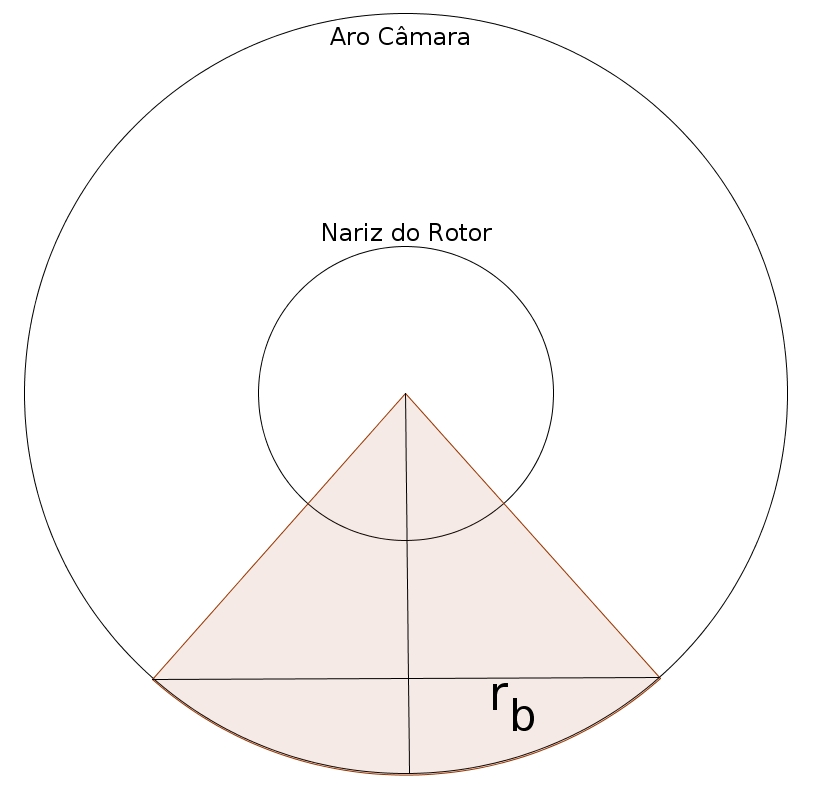
\includegraphics[width=0.9\columnwidth]{figs/base/base_aro_frente.jpg}
	\caption{Visão frontal do aro câmara e raio máximo da base.}
	\label{fig::base_aro_frente}
\end{figure}

O limite superior do raio da base nessa
região é determinado pela região de transição do aro câmara para o tubo de
descarga, onde há uma mudança na inclinação do plano de apoio. A região,
considerada horizontal, que pode acomodar a base do manipulador tem um
comprimento de aproximadamente 1400mm no sentido do fluxo do rio.
Entrentanto, esse limite pode ser contornado construindo-se um plano de apoio
horizontal ou projetando-se a base de forma que ela acompanhe essa
inclinação.É necessário, então, considerar o dimensionamento da base no
cálculo do alcance mínimo do manipulador,que agora se encontra deslocado em
relação à superfície da pá. Sendo assim, alcance mínimo se relaciona com o tamanho do raio da base de 
acordo com $$a_{min}=\sqrt{r_b^2+1800^2}.$$

\begin{figure}[h!]
\centering
	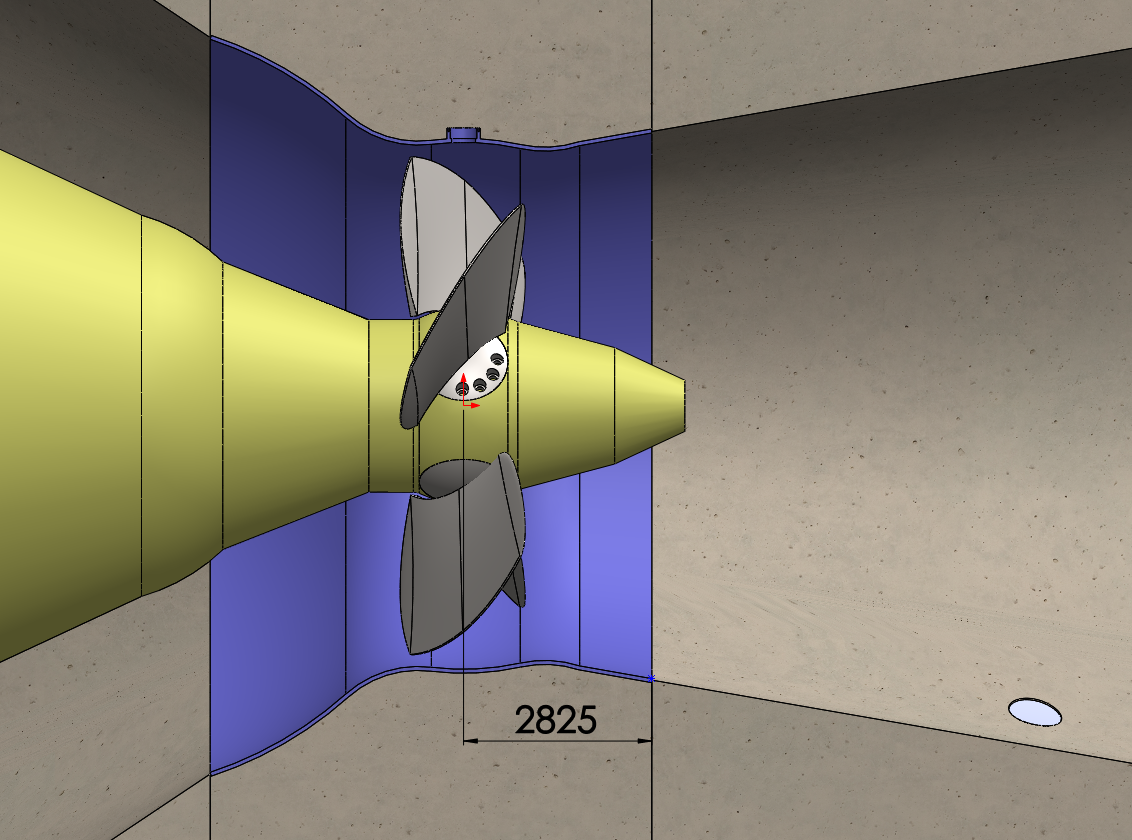
\includegraphics[width=0.9\columnwidth]{figs/base/turbine_side}
	\caption{Visão lateral do aro câmara e raio máximo da base nessa direção.}
	\label{fig::turbine_side}
\end{figure}

O cálculo das dimensões da base com o robô posicionado dentro do aro câmara e
entre as pás, como ilustrado na figura \ref{fig::robot_between}, depende do
ângulo de ataque das pás.

\begin{figure}[h!]
\centering
	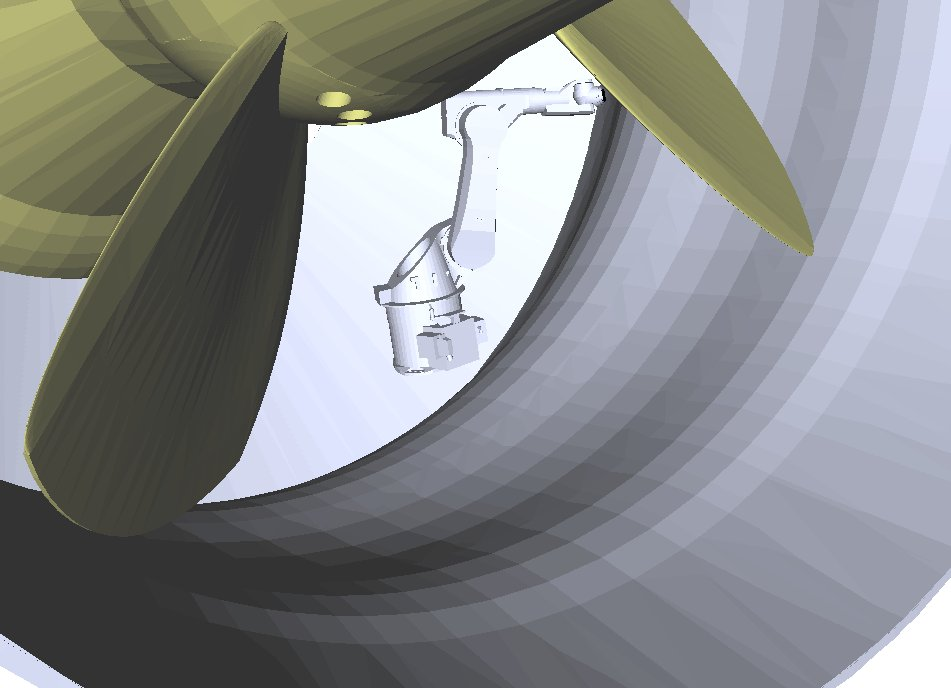
\includegraphics[width=0.9\columnwidth]{figs/openrave/robot_between_openrave.jpg}
	\caption{Exemplo de posicionamento de um manipulador robótico entre as pás.}
	\label{fig::robot_between}
\end{figure}
A distância entre as pás pode ser calculada por meio do cálculo do ângulo diédrico entre elas. A amplitude do movimento de rotação $alpha$ 
das pás é de $14,5^o$ para cada lado a partir da posição zero, entretanto \textbf{essa posição não pôde ser
informada no momento da viagem de reconhecimento e ainda não foi
disponibilizada}. Para critério de cálculos foi utilizado um ângulo de
$45^o$ como a posição de maior abertura das pás e o zero foi considerado como
a reta perpendicular ao fluxo de água. O ângulo diédrico $\theta$ entre as pás
depende do ângulo de ataque das pás e obedece a relação $\cos{\theta} =
\sin^2{\alpha}.$

O a distância entre as pás, considerada como o arco de circunferência no aro
câmara descrito pelo ângulo diédrico calculado, pode ser obtido a partir da
relação $arc=R\alpha$.
Considerando o raio do aro do câmara comoo R=3850mm, o raio máximo da base pode
ser calculado como $$r_{b_e} = (R - h_{b_e})\tan{\theta/2}$$ e com $h_{b_e}$
sendo a altura da base.

O peso mínimo que a base do robô deve possuir está diretamente relacionada com o
tamanho de seu raio. A firgura \ref{fig::tilt_robot} faz uma representação
simplificada da forma que o torque de capotamento máximo atua no robô e em sua
base. Na situação limite, considerando um torque com sentido horário, a força
normal entre a base e a superfície de apoio, $N_2$, teria módulo igual a zero.
No pior caso, podemos considerar que a força vertical exercida pelo robô em sua
base é composta apenas pelo seu peso $W$ e, para que a base não se mova, o
somatório das forças e torques devem ser iguais a zero.

A análise do somatório das forças nos fornece a relação $N_1=W$  e o somatório
dos torques se reduz a $M_k-Wr_b=0$. Sendo assim, a relação entre o raio da base, seu 
peso e o torque máximo de capotamento exercido pelo robô é
da forma 

$$M_k=Wr_b.$$

%TODO refazer figura
\begin{figure}[h!]
\centering
	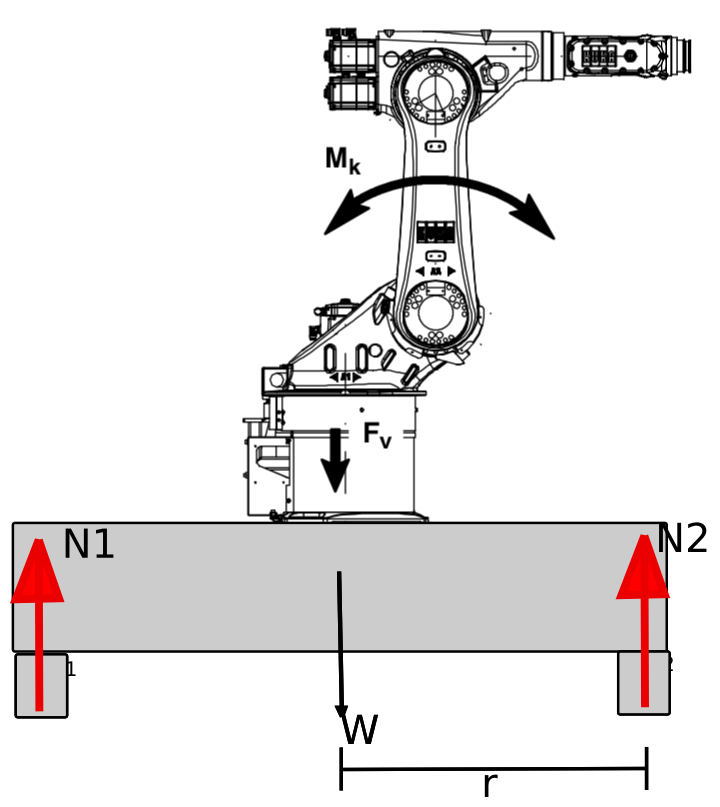
\includegraphics[width=0.5\columnwidth]{figs/base/tilt}
	\caption{Forças e torques máximos entre o robô e sua base.}
	\label{fig::tilt_robot}
\end{figure}

%TODO comparativo entre raio e peso

Uma vez que a superfície do aro câmara e a região adjacente no tubo de sucção
são \textbf{ferromagnéticas}, é possível a utilização de bases magnéticas para
uma compensação do peso e raio necessários para a estabilização do robô. Os
dispositivos magnéticos se dispõem de duas em duas principais catergorias para
essa aplicação:
dispositivos eletretromagnéticos e de imãs permanentes. O primeiro caso tem como
principal vantagem a possibilidade de acionamento remoto, entretanto para situações de
falha em que haja perda de fornecimento de energia, a força de atração também é
perdida. O segundo caso consiste em imãs permanentes arrumados de maneira que
seja possível organizar o seu fluxo magnético e, assim, controlar por meio de
uma alavanca a presença ou ausência de força magnética. A figura
\ref{fig::base::imas} ilustra os dois tipos de bases magnéticas citados.

\begin{figure}[h!]
\begin{subfigure}[b]{0.5\columnwidth}
  \centering
  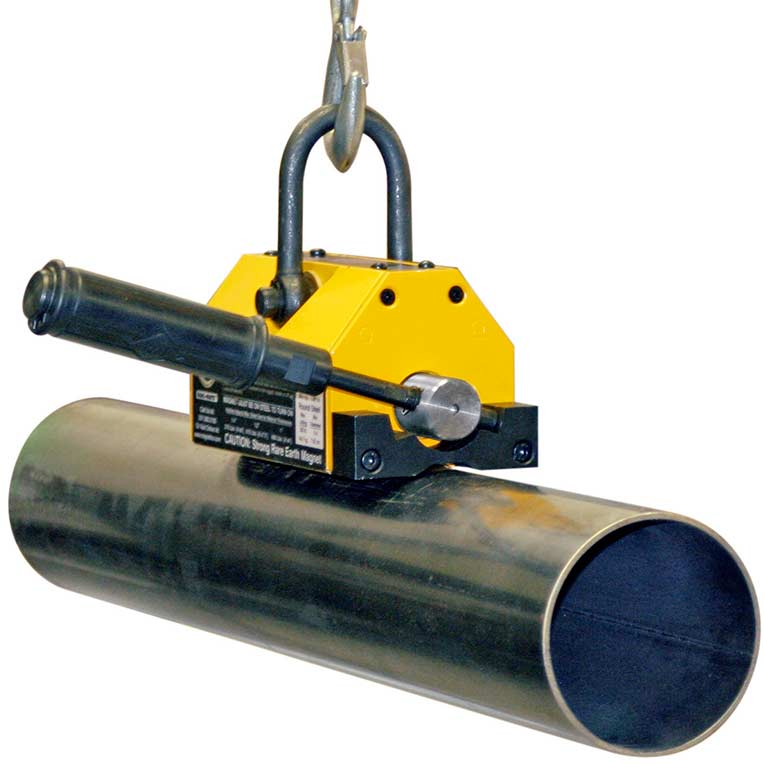
\includegraphics[width=.9\columnwidth]{figs/base/mangnetpipe}
  \caption{Tipo imã permanente}
  \label{fig:sfig1}
\end{subfigure}%
\begin{subfigure}[b]{0.4\columnwidth}
  \centering
  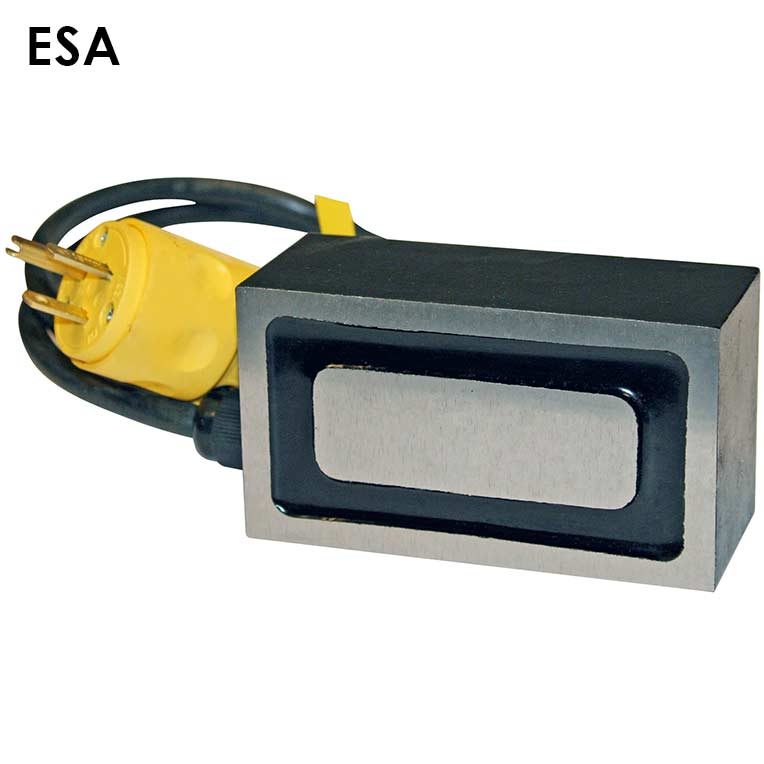
\includegraphics[width=.9\columnwidth]{figs/base/eletromagnet}
  \caption{Tipo eletroimã}
  \label{fig:sfig2}
\end{subfigure}
\caption{Tipos de bases magnéticas comerciais.}
\label{fig::base::imas}
\end{figure}

Comercialmente, foram encontrados bases magnéticas com capacidade de até 3000N.
Um dos requerimentos para a utilização de bases magnéticas, sejam
eletromagnéticas e de imãs permanentes, é a limpeza da superfície de contato
para um acoplamento efeiciente. Essa restrição força a presença humana para a
limpeza e, sobretudo, a verificação de uma correta fixação. Sendo assim, as
bases magnéticas de imã permanente se mostram mais coerentes para a aplicação,
pois não possuem ponto de falha para o caso de perda de energia do sistema e
possuem uma maior capacidade de carga. A curvatura do ambiente não é um
limitante, sendo possível até a confecção de uma máscara para a base de maneira
que a superfície de apoio se conforme perfeitamente com a superfície de fixação.

\subsection{Estudo de anteparo de proteção para a chama}
Quando não é possível, em uma passada única, atraves\-sar completamente a
superfície da pá ao realizar o revestimento, coloca-se uma placa de sacrifício,
pois, como menciona\-do em \ref{sec::desc_hvof}, não é permitido parar ou trocar
de direção sobre a superfície.

Para evitar a necessidade de sobrepor placas de sacrifício sobre as pás da
turbina, que podem estar em posição de difícil acesso, foi criado o conceito de
\textit{shutter}. Este consiste em um anteparo a ser posicionado entre a chama e
a superfície, porém, diferente da placa de sacrifício, deve ficar preso à
pistola de metalização e ser atuado.

A pistola de metalização propaga uma chama de $3000^o$ (\ref{sec::desc_hvof}),
logo a parte da pistola com maior aquecimento, que é o canhão, é fabricado em
cobre-cromo e é refrigerada por um sistema de circulação de água
gelada. A chapa de sacrifício, por outro lado, fica pouco tempo em contato com
a chama e é constituída de um aço qualquer sem sistema de refrigeração
\ref{sec::desc_hvof}.

Quando se planeja submeter o anteparo à temperatu\-ra extrema de $3000^o$ da
chama, sem um sistema de refrigeração, torna-se necessário o uso de materia\-is
especiais para suportar essa temperatura. Para isso existem materiais
aeroespaciais, conhecidos como Ultra-high-temperature ceramics (UHTCs) ou
cerâmi\-cas de temperaturas ultra-altas, em tradução livre. Esse grupo de
materiais possui diversas subfamílias com densidades e resistência mecânicas
diferentes. Para os cálculos realizados nessa seção foram consideradas a maior
densidade e menor resistência mecânica entre os compostos das sub-famílias. Ou
seja, foi utilizado aproximadamente \textbf{$15 g/mL$} para a densidade, referente ao
carbeto de tântalo \citep{bansal2005ceramic}. E as características mecânicas
foram referentes ao diboreto de zircônio \citep{diborides}.

Foram desenvolvidos dois conceitos similares para resolver o problema, o \textit{Shutter
Borboleta} e o \textit{Shutter Padrão}, descritos a seguir.

\subsubsection{\textit{Shutter} Borboleta}
\label{borboleta}

Esse primeiro conceito é constituído de um disco disposto entre a chama e a
superfície. O disco possui duas aberturas opostas de $90^o$, por onde a chama da
pistola atravessa, e as outras duas regiões compostas pelo material
aeroespacial que servirá de anteparo para a chama, evitando o
revestimento da superfície. A disposição do material dá o nome
``borboleta'' ao design.

O disco é suportado por um eixo que é rotacionado por um motor fixado sobre o
corpo da pistola de metalização (figuras \ref{fig::borboleta_aberta} e
\ref{fig::borboleta_fechada}).

\begin{figure}[h!]
\centering
	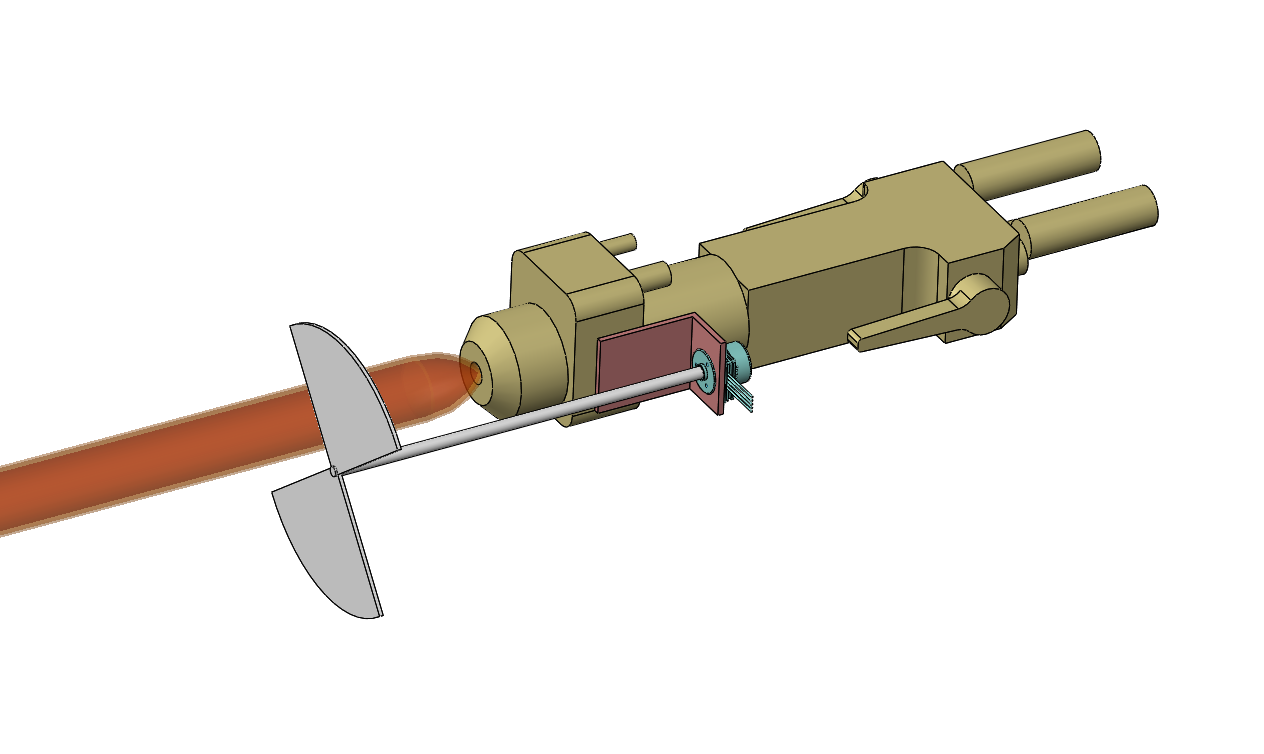
\includegraphics[width=\columnwidth]{figs/estudo/shutter/Shutter_Borboleta_Aberto}
	\caption{\textit{Shutter} Borboleta em posição aberta, permitindo a passagem da chama
	de coating.}
	\label{fig::borboleta_aberta}
\end{figure}

Quando uma das regiões de abertura do \textit{shutter} se encontra na direção da
chama (figura \ref{fig::borboleta_aberta}), esta o atravessa e atinge a
superfície a ser tratada sem sofrer desvios. Para realizar uma mudança de
direção do revestimento ou parada por qualquer motivo, o motor gira o conjunto
eixo/disco e posiciona a região de proteção na direção da chama, o que impede a passagem da
chama (figura \ref{fig::borboleta_fechada}).

\begin{figure}[h!]
\centering
	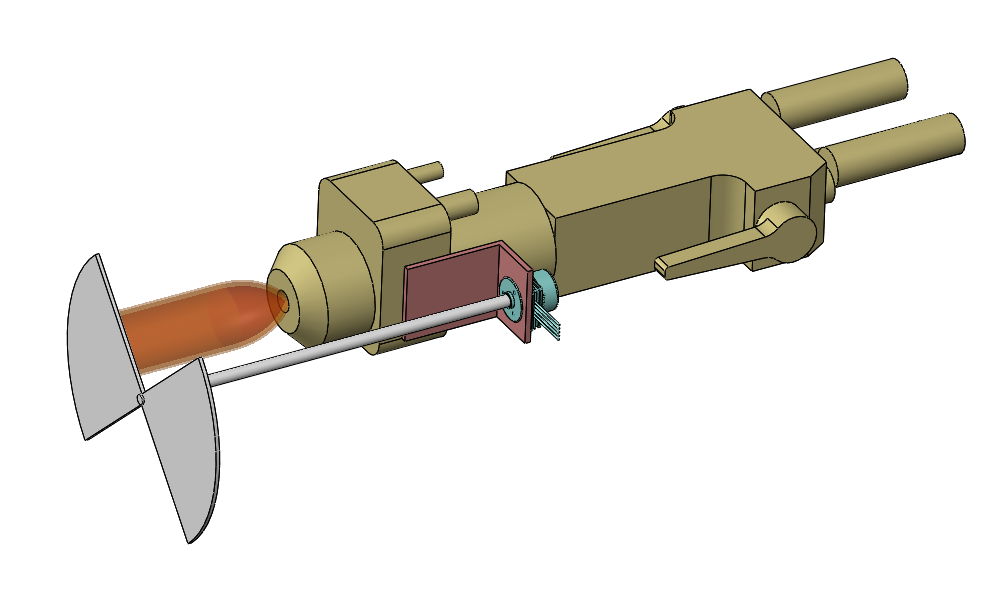
\includegraphics[width=\columnwidth]{figs/estudo/shutter/Shutter_Borboleta_Fechado}
	\caption{\textit{Shutter} Borboleta em posição fechada, evitando a passagem da chama
	de coating, agindo como anteparo de forma similar à chapa de sacrifício.}
	\label{fig::borboleta_fechada}
\end{figure}

Para dimensionamento do eixo e da borboleta foram considerados os seguintes
parâmetros:

\[\rho = 15 g/mL\]
\[v_{close} = 40 m/min\]
\[d_{flame} = 33mm\]
\[L = 20mm\]

Onde $\rho$ é a densidade do material do \textit{shutter}, $v_{close}$ a
velocidade de fechamento sobre a chama, $d_{flame}$ o diâmetro da chama e $L$ o
comprimento do eixo. Além desses parâmetros, foram utilizadas informações
mecânicas como módulos de elasticidade e limites de escoamentos típicos de aço.

Para a escolha do comprimento do eixo, o objetivo foi posicionar o
\textit{shutter} a meio caminho da pistola à superfície, e mantendo $10cm$ de
distância entre a posição do motor e a saída da chama (a fim de evitar
exposição ao calor intenso). Durante o dimensionamento do shutter foi
considerado um valor de segurança para o diâmetro da chama como o dobro do
diâmetro real.

A partir desses dados chegamos aos seguintes requisitos para o sistema:

\[ r = 80 mm\]
\[ \epsilon = 5 mm\]
\[ \omega = 160 rpm\]
\[ {Pot}_{min} = 5 W \]
\[ \tau_{min} = 420 mNm \]
\[ Pot_{\tau} = 7 W \]
\[ d_{eixo} = 7 mm\]

Onde $r$ é o raio do \textit{shutter}, $\epsilon$ sua espessura, o que acarreta
um peso de $750 g$ para o \textit{shutter}.

Há, também, $\omega$ que é a velocidade de rotação que o motor precisa alcançar,
$Pot_{min}$ sua potência mínima e $\tau_{min}$ seu torque mínimo necessário.
$Pot_{\tau}$ é a potência mínima necessária caso o torque mínimo ($\tau_{min}$)
for mantido durante todo o percurso. E, por fim, $\d_{eixo}$ é o diâmetro necessário do eixo para suportar a
pressão da chama.

Foram pesquisados motores industriais de pequenas dimensões (menos de 300 g),
porém não foram encontrados motores capazes de suprir o torque necessário. Como
são facilmente encontrados motores que satisfazem as restrições de potência,
existem redutores de dimensões diminutas que podem ser acoplados ao motor para
fazê-lo trabalhar na faixa de torque necessária.


\subsubsection{Shutter Padrão}

O \textit{Shutter} Padrão é composto por uma pequena chapa quadrada que é
posicionada entre a pistola e a superfície pela atuação de um motor. O motor é
conectado à chapa por quatro hastes presas em suas extremidades, como mostram as
figuras \ref{fig::padrao_aberto} e \ref{fig::padrao_fechado}.

\begin{figure}[h!]
\centering
	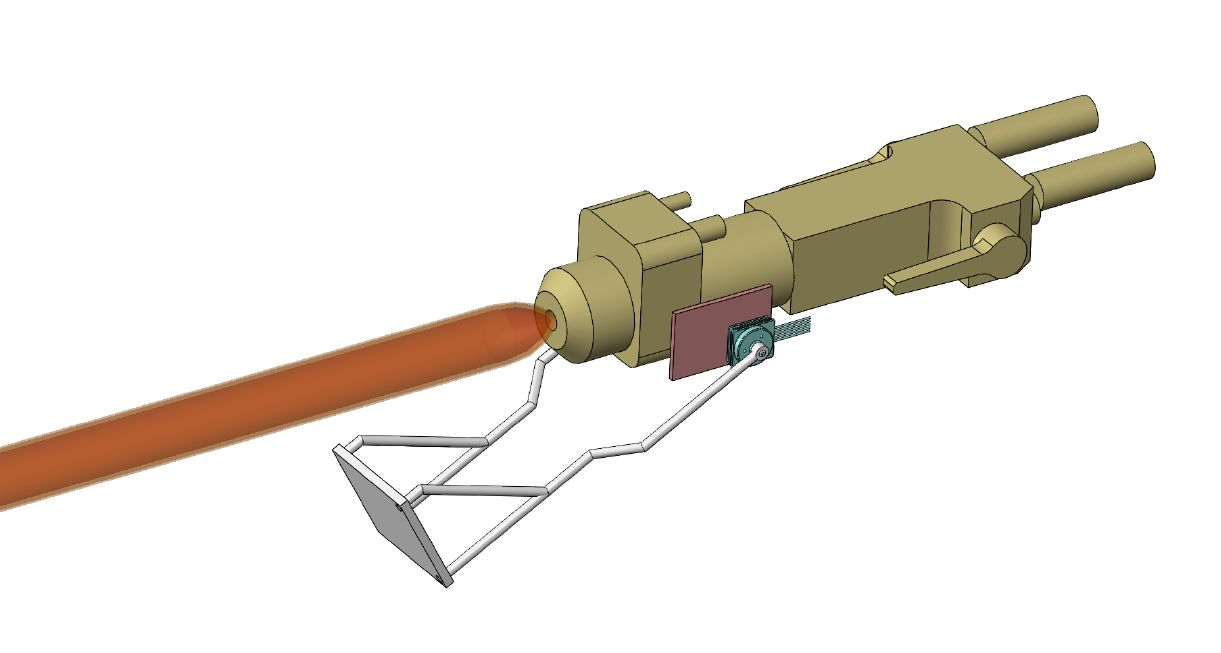
\includegraphics[width=\columnwidth]{figs/estudo/shutter/Padrao_aberto}
	\caption{\textit{Shutter} Padrão em posição aberta, permitindo a passagem da chama
	de coating.}
	\label{fig::padrao_aberto}
\end{figure}

Quando a chapa se encontra fora do eixo da chama dizemos que
o \textit{shutter} está aberto (figura \ref{fig::padrao_aberto}), permitindo que
o revestimento seja realizado normalmente. Na necessidade de impedir a
passagem da chama, o motor atua sobre as hastes guiando a chapa para servir de
anteparo à chama (figura \ref{fig::padrao_fechado}).

\begin{figure}[h!]
\centering
	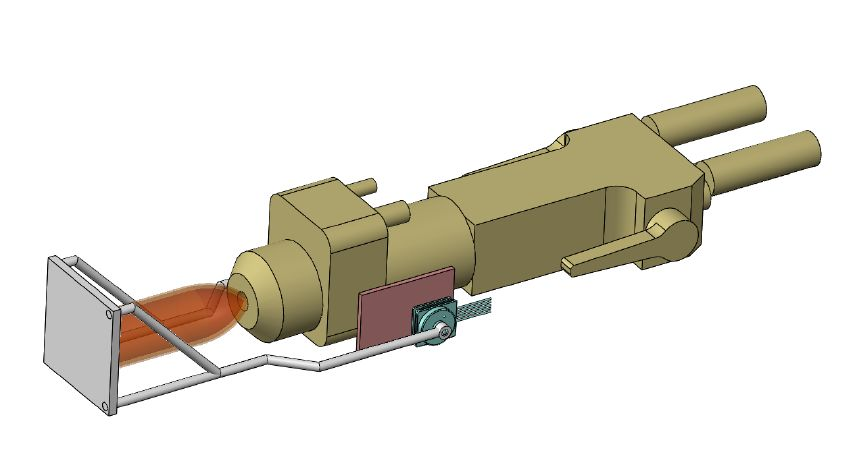
\includegraphics[width=\columnwidth]{figs/estudo/shutter/Padrao_fechado}
	\caption{\textit{Shutter} Padrão em posição fechada, evitando a passagem da
	chama de coating, agindo como anteparo de forma similar à chapa de sacrifício.}
	\label{fig::padrao_fechado}
\end{figure}

Para calcular os requisitos do motor e da chapa foram considerados os mesmos
valores utilizados no \textit{shutter} borboleta (\ref{borboleta}). Sendo a
escolha do comprimento do eixo e o diâmetro de segurança da chama feitos
seguindo os mesmo preceitos também lá descritos.

A partir desses dados chegamos aos seguintes requisitos para o sistema:

\[ l = 66 mm\]
\[ \epsilon = 5 mm\]
\[ \omega = 32 rpm\]
\[ {Pot}_{min} = 2 W \]
\[ \tau_{min} = 920 mNm \]
\[ Pot_{\tau} = 3 W \]


Onde $l$ é o lado da chapa do \textit{shutter}, $\epsilon$ sua espessura, o que
acarreta um peso de $350 g$ para o \textit{shutter}.

A velocidade de rotação que o motor precisa alcançar foi nomeada $\omega$, sua
potência mínima $Pot_{min}$  e seu torque mínimo necessário $\tau_{min}$.
$Pot_{\tau}$ é a potência mínima necessária para que o torque mínimo
($\tau_{min}$) consiga ser mantido durante todo o percurso de fechar/abrir.

Assim como para o \textit{shutter} borboleta não foram encontrados motores
capazes de suprir o torque necessário. E a solução pelo uso de redutores de
dimensões diminutas pode ser facilmente aplicada devido à baixa potência
requerida.
 
\section{Conclusão e trabalhos futuros}\label{sec:conclusions}
  
\bibliography{main} 
\appendix
\end{document}
